\documentclass{article}
\usepackage{iclr2027_conference,times}

%%%%% NEW MATH DEFINITIONS %%%%%

\usepackage{amsmath,amsfonts,bm}

% Mark sections of captions for referring to divisions of figures
\newcommand{\figleft}{{\em (Left)}}
\newcommand{\figcenter}{{\em (Center)}}
\newcommand{\figright}{{\em (Right)}}
\newcommand{\figtop}{{\em (Top)}}
\newcommand{\figbottom}{{\em (Bottom)}}
\newcommand{\captiona}{{\em (a)}}
\newcommand{\captionb}{{\em (b)}}
\newcommand{\captionc}{{\em (c)}}
\newcommand{\captiond}{{\em (d)}}

% Highlight a newly defined term
\newcommand{\newterm}[1]{{\bf #1}}


% Figure reference, lower-case.
\def\figref#1{figure~\ref{#1}}
% Figure reference, capital. For start of sentence
\def\Figref#1{Figure~\ref{#1}}
\def\twofigref#1#2{figures \ref{#1} and \ref{#2}}
\def\quadfigref#1#2#3#4{figures \ref{#1}, \ref{#2}, \ref{#3} and \ref{#4}}
% Section reference, lower-case.
\def\secref#1{section~\ref{#1}}
% Section reference, capital.
\def\Secref#1{Section~\ref{#1}}
% Reference to two sections.
\def\twosecrefs#1#2{sections \ref{#1} and \ref{#2}}
% Reference to three sections.
\def\secrefs#1#2#3{sections \ref{#1}, \ref{#2} and \ref{#3}}
% Reference to an equation, lower-case.
\def\eqref#1{equation~\ref{#1}}
% Reference to an equation, upper case
\def\Eqref#1{Equation~\ref{#1}}
% A raw reference to an equation---avoid using if possible
\def\plaineqref#1{\ref{#1}}
% Reference to a chapter, lower-case.
\def\chapref#1{chapter~\ref{#1}}
% Reference to an equation, upper case.
\def\Chapref#1{Chapter~\ref{#1}}
% Reference to a range of chapters
\def\rangechapref#1#2{chapters\ref{#1}--\ref{#2}}
% Reference to an algorithm, lower-case.
\def\algref#1{algorithm~\ref{#1}}
% Reference to an algorithm, upper case.
\def\Algref#1{Algorithm~\ref{#1}}
\def\twoalgref#1#2{algorithms \ref{#1} and \ref{#2}}
\def\Twoalgref#1#2{Algorithms \ref{#1} and \ref{#2}}
% Reference to a part, lower case
\def\partref#1{part~\ref{#1}}
% Reference to a part, upper case
\def\Partref#1{Part~\ref{#1}}
\def\twopartref#1#2{parts \ref{#1} and \ref{#2}}

\def\ceil#1{\lceil #1 \rceil}
\def\floor#1{\lfloor #1 \rfloor}
\def\1{\bm{1}}
\newcommand{\train}{\mathcal{D}}
\newcommand{\valid}{\mathcal{D_{\mathrm{valid}}}}
\newcommand{\test}{\mathcal{D_{\mathrm{test}}}}

\def\eps{{\epsilon}}


% Random variables
\def\reta{{\textnormal{$\eta$}}}
\def\ra{{\textnormal{a}}}
\def\rb{{\textnormal{b}}}
\def\rc{{\textnormal{c}}}
\def\rd{{\textnormal{d}}}
\def\re{{\textnormal{e}}}
\def\rf{{\textnormal{f}}}
\def\rg{{\textnormal{g}}}
\def\rh{{\textnormal{h}}}
\def\ri{{\textnormal{i}}}
\def\rj{{\textnormal{j}}}
\def\rk{{\textnormal{k}}}
\def\rl{{\textnormal{l}}}
% rm is already a command, just don't name any random variables m
\def\rn{{\textnormal{n}}}
\def\ro{{\textnormal{o}}}
\def\rp{{\textnormal{p}}}
\def\rq{{\textnormal{q}}}
\def\rr{{\textnormal{r}}}
\def\rs{{\textnormal{s}}}
\def\rt{{\textnormal{t}}}
\def\ru{{\textnormal{u}}}
\def\rv{{\textnormal{v}}}
\def\rw{{\textnormal{w}}}
\def\rx{{\textnormal{x}}}
\def\ry{{\textnormal{y}}}
\def\rz{{\textnormal{z}}}

% Random vectors
\def\rvepsilon{{\mathbf{\epsilon}}}
\def\rvtheta{{\mathbf{\theta}}}
\def\rva{{\mathbf{a}}}
\def\rvb{{\mathbf{b}}}
\def\rvc{{\mathbf{c}}}
\def\rvd{{\mathbf{d}}}
\def\rve{{\mathbf{e}}}
\def\rvf{{\mathbf{f}}}
\def\rvg{{\mathbf{g}}}
\def\rvh{{\mathbf{h}}}
\def\rvu{{\mathbf{i}}}
\def\rvj{{\mathbf{j}}}
\def\rvk{{\mathbf{k}}}
\def\rvl{{\mathbf{l}}}
\def\rvm{{\mathbf{m}}}
\def\rvn{{\mathbf{n}}}
\def\rvo{{\mathbf{o}}}
\def\rvp{{\mathbf{p}}}
\def\rvq{{\mathbf{q}}}
\def\rvr{{\mathbf{r}}}
\def\rvs{{\mathbf{s}}}
\def\rvt{{\mathbf{t}}}
\def\rvu{{\mathbf{u}}}
\def\rvv{{\mathbf{v}}}
\def\rvw{{\mathbf{w}}}
\def\rvx{{\mathbf{x}}}
\def\rvy{{\mathbf{y}}}
\def\rvz{{\mathbf{z}}}

% Elements of random vectors
\def\erva{{\textnormal{a}}}
\def\ervb{{\textnormal{b}}}
\def\ervc{{\textnormal{c}}}
\def\ervd{{\textnormal{d}}}
\def\erve{{\textnormal{e}}}
\def\ervf{{\textnormal{f}}}
\def\ervg{{\textnormal{g}}}
\def\ervh{{\textnormal{h}}}
\def\ervi{{\textnormal{i}}}
\def\ervj{{\textnormal{j}}}
\def\ervk{{\textnormal{k}}}
\def\ervl{{\textnormal{l}}}
\def\ervm{{\textnormal{m}}}
\def\ervn{{\textnormal{n}}}
\def\ervo{{\textnormal{o}}}
\def\ervp{{\textnormal{p}}}
\def\ervq{{\textnormal{q}}}
\def\ervr{{\textnormal{r}}}
\def\ervs{{\textnormal{s}}}
\def\ervt{{\textnormal{t}}}
\def\ervu{{\textnormal{u}}}
\def\ervv{{\textnormal{v}}}
\def\ervw{{\textnormal{w}}}
\def\ervx{{\textnormal{x}}}
\def\ervy{{\textnormal{y}}}
\def\ervz{{\textnormal{z}}}

% Random matrices
\def\rmA{{\mathbf{A}}}
\def\rmB{{\mathbf{B}}}
\def\rmC{{\mathbf{C}}}
\def\rmD{{\mathbf{D}}}
\def\rmE{{\mathbf{E}}}
\def\rmF{{\mathbf{F}}}
\def\rmG{{\mathbf{G}}}
\def\rmH{{\mathbf{H}}}
\def\rmI{{\mathbf{I}}}
\def\rmJ{{\mathbf{J}}}
\def\rmK{{\mathbf{K}}}
\def\rmL{{\mathbf{L}}}
\def\rmM{{\mathbf{M}}}
\def\rmN{{\mathbf{N}}}
\def\rmO{{\mathbf{O}}}
\def\rmP{{\mathbf{P}}}
\def\rmQ{{\mathbf{Q}}}
\def\rmR{{\mathbf{R}}}
\def\rmS{{\mathbf{S}}}
\def\rmT{{\mathbf{T}}}
\def\rmU{{\mathbf{U}}}
\def\rmV{{\mathbf{V}}}
\def\rmW{{\mathbf{W}}}
\def\rmX{{\mathbf{X}}}
\def\rmY{{\mathbf{Y}}}
\def\rmZ{{\mathbf{Z}}}

% Elements of random matrices
\def\ermA{{\textnormal{A}}}
\def\ermB{{\textnormal{B}}}
\def\ermC{{\textnormal{C}}}
\def\ermD{{\textnormal{D}}}
\def\ermE{{\textnormal{E}}}
\def\ermF{{\textnormal{F}}}
\def\ermG{{\textnormal{G}}}
\def\ermH{{\textnormal{H}}}
\def\ermI{{\textnormal{I}}}
\def\ermJ{{\textnormal{J}}}
\def\ermK{{\textnormal{K}}}
\def\ermL{{\textnormal{L}}}
\def\ermM{{\textnormal{M}}}
\def\ermN{{\textnormal{N}}}
\def\ermO{{\textnormal{O}}}
\def\ermP{{\textnormal{P}}}
\def\ermQ{{\textnormal{Q}}}
\def\ermR{{\textnormal{R}}}
\def\ermS{{\textnormal{S}}}
\def\ermT{{\textnormal{T}}}
\def\ermU{{\textnormal{U}}}
\def\ermV{{\textnormal{V}}}
\def\ermW{{\textnormal{W}}}
\def\ermX{{\textnormal{X}}}
\def\ermY{{\textnormal{Y}}}
\def\ermZ{{\textnormal{Z}}}

% Vectors
\def\vzero{{\bm{0}}}
\def\vone{{\bm{1}}}
\def\vmu{{\bm{\mu}}}
\def\vtheta{{\bm{\theta}}}
\def\va{{\bm{a}}}
\def\vb{{\bm{b}}}
\def\vc{{\bm{c}}}
\def\vd{{\bm{d}}}
\def\ve{{\bm{e}}}
\def\vf{{\bm{f}}}
\def\vg{{\bm{g}}}
\def\vh{{\bm{h}}}
\def\vi{{\bm{i}}}
\def\vj{{\bm{j}}}
\def\vk{{\bm{k}}}
\def\vl{{\bm{l}}}
\def\vm{{\bm{m}}}
\def\vn{{\bm{n}}}
\def\vo{{\bm{o}}}
\def\vp{{\bm{p}}}
\def\vq{{\bm{q}}}
\def\vr{{\bm{r}}}
\def\vs{{\bm{s}}}
\def\vt{{\bm{t}}}
\def\vu{{\bm{u}}}
\def\vv{{\bm{v}}}
\def\vw{{\bm{w}}}
\def\vx{{\bm{x}}}
\def\vy{{\bm{y}}}
\def\vz{{\bm{z}}}

% Elements of vectors
\def\evalpha{{\alpha}}
\def\evbeta{{\beta}}
\def\evepsilon{{\epsilon}}
\def\evlambda{{\lambda}}
\def\evomega{{\omega}}
\def\evmu{{\mu}}
\def\evpsi{{\psi}}
\def\evsigma{{\sigma}}
\def\evtheta{{\theta}}
\def\eva{{a}}
\def\evb{{b}}
\def\evc{{c}}
\def\evd{{d}}
\def\eve{{e}}
\def\evf{{f}}
\def\evg{{g}}
\def\evh{{h}}
\def\evi{{i}}
\def\evj{{j}}
\def\evk{{k}}
\def\evl{{l}}
\def\evm{{m}}
\def\evn{{n}}
\def\evo{{o}}
\def\evp{{p}}
\def\evq{{q}}
\def\evr{{r}}
\def\evs{{s}}
\def\evt{{t}}
\def\evu{{u}}
\def\evv{{v}}
\def\evw{{w}}
\def\evx{{x}}
\def\evy{{y}}
\def\evz{{z}}

% Matrix
\def\mA{{\bm{A}}}
\def\mB{{\bm{B}}}
\def\mC{{\bm{C}}}
\def\mD{{\bm{D}}}
\def\mE{{\bm{E}}}
\def\mF{{\bm{F}}}
\def\mG{{\bm{G}}}
\def\mH{{\bm{H}}}
\def\mI{{\bm{I}}}
\def\mJ{{\bm{J}}}
\def\mK{{\bm{K}}}
\def\mL{{\bm{L}}}
\def\mM{{\bm{M}}}
\def\mN{{\bm{N}}}
\def\mO{{\bm{O}}}
\def\mP{{\bm{P}}}
\def\mQ{{\bm{Q}}}
\def\mR{{\bm{R}}}
\def\mS{{\bm{S}}}
\def\mT{{\bm{T}}}
\def\mU{{\bm{U}}}
\def\mV{{\bm{V}}}
\def\mW{{\bm{W}}}
\def\mX{{\bm{X}}}
\def\mY{{\bm{Y}}}
\def\mZ{{\bm{Z}}}
\def\mBeta{{\bm{\beta}}}
\def\mPhi{{\bm{\Phi}}}
\def\mLambda{{\bm{\Lambda}}}
\def\mSigma{{\bm{\Sigma}}}

% Tensor
\DeclareMathAlphabet{\mathsfit}{\encodingdefault}{\sfdefault}{m}{sl}
\SetMathAlphabet{\mathsfit}{bold}{\encodingdefault}{\sfdefault}{bx}{n}
\newcommand{\tens}[1]{\bm{\mathsfit{#1}}}
\def\tA{{\tens{A}}}
\def\tB{{\tens{B}}}
\def\tC{{\tens{C}}}
\def\tD{{\tens{D}}}
\def\tE{{\tens{E}}}
\def\tF{{\tens{F}}}
\def\tG{{\tens{G}}}
\def\tH{{\tens{H}}}
\def\tI{{\tens{I}}}
\def\tJ{{\tens{J}}}
\def\tK{{\tens{K}}}
\def\tL{{\tens{L}}}
\def\tM{{\tens{M}}}
\def\tN{{\tens{N}}}
\def\tO{{\tens{O}}}
\def\tP{{\tens{P}}}
\def\tQ{{\tens{Q}}}
\def\tR{{\tens{R}}}
\def\tS{{\tens{S}}}
\def\tT{{\tens{T}}}
\def\tU{{\tens{U}}}
\def\tV{{\tens{V}}}
\def\tW{{\tens{W}}}
\def\tX{{\tens{X}}}
\def\tY{{\tens{Y}}}
\def\tZ{{\tens{Z}}}


% Graph
\def\gA{{\mathcal{A}}}
\def\gB{{\mathcal{B}}}
\def\gC{{\mathcal{C}}}
\def\gD{{\mathcal{D}}}
\def\gE{{\mathcal{E}}}
\def\gF{{\mathcal{F}}}
\def\gG{{\mathcal{G}}}
\def\gH{{\mathcal{H}}}
\def\gI{{\mathcal{I}}}
\def\gJ{{\mathcal{J}}}
\def\gK{{\mathcal{K}}}
\def\gL{{\mathcal{L}}}
\def\gM{{\mathcal{M}}}
\def\gN{{\mathcal{N}}}
\def\gO{{\mathcal{O}}}
\def\gP{{\mathcal{P}}}
\def\gQ{{\mathcal{Q}}}
\def\gR{{\mathcal{R}}}
\def\gS{{\mathcal{S}}}
\def\gT{{\mathcal{T}}}
\def\gU{{\mathcal{U}}}
\def\gV{{\mathcal{V}}}
\def\gW{{\mathcal{W}}}
\def\gX{{\mathcal{X}}}
\def\gY{{\mathcal{Y}}}
\def\gZ{{\mathcal{Z}}}

% Sets
\def\sA{{\mathbb{A}}}
\def\sB{{\mathbb{B}}}
\def\sC{{\mathbb{C}}}
\def\sD{{\mathbb{D}}}
% Don't use a set called E, because this would be the same as our symbol
% for expectation.
\def\sF{{\mathbb{F}}}
\def\sG{{\mathbb{G}}}
\def\sH{{\mathbb{H}}}
\def\sI{{\mathbb{I}}}
\def\sJ{{\mathbb{J}}}
\def\sK{{\mathbb{K}}}
\def\sL{{\mathbb{L}}}
\def\sM{{\mathbb{M}}}
\def\sN{{\mathbb{N}}}
\def\sO{{\mathbb{O}}}
\def\sP{{\mathbb{P}}}
\def\sQ{{\mathbb{Q}}}
\def\sR{{\mathbb{R}}}
\def\sS{{\mathbb{S}}}
\def\sT{{\mathbb{T}}}
\def\sU{{\mathbb{U}}}
\def\sV{{\mathbb{V}}}
\def\sW{{\mathbb{W}}}
\def\sX{{\mathbb{X}}}
\def\sY{{\mathbb{Y}}}
\def\sZ{{\mathbb{Z}}}

% Entries of a matrix
\def\emLambda{{\Lambda}}
\def\emA{{A}}
\def\emB{{B}}
\def\emC{{C}}
\def\emD{{D}}
\def\emE{{E}}
\def\emF{{F}}
\def\emG{{G}}
\def\emH{{H}}
\def\emI{{I}}
\def\emJ{{J}}
\def\emK{{K}}
\def\emL{{L}}
\def\emM{{M}}
\def\emN{{N}}
\def\emO{{O}}
\def\emP{{P}}
\def\emQ{{Q}}
\def\emR{{R}}
\def\emS{{S}}
\def\emT{{T}}
\def\emU{{U}}
\def\emV{{V}}
\def\emW{{W}}
\def\emX{{X}}
\def\emY{{Y}}
\def\emZ{{Z}}
\def\emSigma{{\Sigma}}

% entries of a tensor
% Same font as tensor, without \bm wrapper
\newcommand{\etens}[1]{\mathsfit{#1}}
\def\etLambda{{\etens{\Lambda}}}
\def\etA{{\etens{A}}}
\def\etB{{\etens{B}}}
\def\etC{{\etens{C}}}
\def\etD{{\etens{D}}}
\def\etE{{\etens{E}}}
\def\etF{{\etens{F}}}
\def\etG{{\etens{G}}}
\def\etH{{\etens{H}}}
\def\etI{{\etens{I}}}
\def\etJ{{\etens{J}}}
\def\etK{{\etens{K}}}
\def\etL{{\etens{L}}}
\def\etM{{\etens{M}}}
\def\etN{{\etens{N}}}
\def\etO{{\etens{O}}}
\def\etP{{\etens{P}}}
\def\etQ{{\etens{Q}}}
\def\etR{{\etens{R}}}
\def\etS{{\etens{S}}}
\def\etT{{\etens{T}}}
\def\etU{{\etens{U}}}
\def\etV{{\etens{V}}}
\def\etW{{\etens{W}}}
\def\etX{{\etens{X}}}
\def\etY{{\etens{Y}}}
\def\etZ{{\etens{Z}}}

% The true underlying data generating distribution
\newcommand{\pdata}{p_{\rm{data}}}
% The empirical distribution defined by the training set
\newcommand{\ptrain}{\hat{p}_{\rm{data}}}
\newcommand{\Ptrain}{\hat{P}_{\rm{data}}}
% The model distribution
\newcommand{\pmodel}{p_{\rm{model}}}
\newcommand{\Pmodel}{P_{\rm{model}}}
\newcommand{\ptildemodel}{\tilde{p}_{\rm{model}}}
% Stochastic autoencoder distributions
\newcommand{\pencode}{p_{\rm{encoder}}}
\newcommand{\pdecode}{p_{\rm{decoder}}}
\newcommand{\precons}{p_{\rm{reconstruct}}}

\newcommand{\laplace}{\mathrm{Laplace}} % Laplace distribution

\newcommand{\E}{\mathbb{E}}
\newcommand{\Ls}{\mathcal{L}}
\newcommand{\R}{\mathbb{R}}
\newcommand{\emp}{\tilde{p}}
\newcommand{\lr}{\alpha}
\newcommand{\reg}{\lambda}
\newcommand{\rect}{\mathrm{rectifier}}
\newcommand{\softmax}{\mathrm{softmax}}
\newcommand{\sigmoid}{\sigma}
\newcommand{\softplus}{\zeta}
\newcommand{\KL}{D_{\mathrm{KL}}}
\newcommand{\Var}{\mathrm{Var}}
\newcommand{\standarderror}{\mathrm{SE}}
\newcommand{\Cov}{\mathrm{Cov}}
% Wolfram Mathworld says $L^2$ is for function spaces and $\ell^2$ is for vectors
% But then they seem to use $L^2$ for vectors throughout the site, and so does
% wikipedia.
\newcommand{\normlzero}{L^0}
\newcommand{\normlone}{L^1}
\newcommand{\normltwo}{L^2}
\newcommand{\normlp}{L^p}
\newcommand{\normmax}{L^\infty}

\newcommand{\parents}{Pa} % See usage in notation.tex. Chosen to match Daphne's book.

\DeclareMathOperator*{\argmax}{arg\,max}
\DeclareMathOperator*{\argmin}{arg\,min}

\DeclareMathOperator{\sign}{sign}
\DeclareMathOperator{\Tr}{Tr}
\let\ab\allowbreak


\usepackage{url}
\usepackage{booktabs}
\usepackage{graphicx}
\usepackage{amsmath}
\usepackage{amsthm}
\newtheorem{lemma}{Lemma}
\usepackage{amssymb}
\usepackage{xcolor}
\usepackage{multirow}
\usepackage{enumitem}
\usepackage{csquotes}   % \enquote{...} -- nested-aware, locale-correct quotes
\usepackage{acronym}    % \acro/\ac -- see note below

% hyperref wants to be loaded after almost everything else, and cleveref is the
% one package that must be loaded after hyperref. Do not reorder these two.
% backref=page appends the citing page(s) to each bibliography entry.
\usepackage[backref=page]{hyperref}
\usepackage{cleveref}

% Without this, backref renders the citing page as a bare digit butted against
% the year ("... (ICML), 2018. 3"), which reads like part of the reference.
\renewcommand*{\backref}[1]{}
\renewcommand*{\backrefalt}[4]{%
  \ifcase #1 %
  \or \ (cited on page #2)%
  \else \ (cited on pages #2)%
  \fi}

% A little slack for lines TeX cannot break well (long \texttt identifiers and
% math runs inside tight list items). Without it those lines overflow into the
% margin rather than stretching.
\emergencystretch=1.5em

% ---------------------------------------------------------------------------
% Float packing. The defaults reserve so much of each page for text that a page
% carrying one figure wastes a third of its height. These are the standard
% loosenings; they change no layout rule the style file sets, only how much of a
% page a float may claim before LaTeX gives up and defers it.
% ---------------------------------------------------------------------------
\renewcommand{\topfraction}{0.92}
\renewcommand{\bottomfraction}{0.75}
\renewcommand{\textfraction}{0.07}
\renewcommand{\floatpagefraction}{0.80}
\setcounter{topnumber}{3}
\setcounter{bottomnumber}{2}
\setcounter{totalnumber}{4}

% ---------------------------------------------------------------------------
% Drafting aids. \TODO renders loudly on purpose: anything still marked when
% the PDF is built is something that has not been measured yet, and the point
% is that it cannot be missed. Set \draftfalse before submitting -- the build
% then errors on any remaining \TODO rather than hiding it.
% ---------------------------------------------------------------------------
\newif\ifdraft\drafttrue
\ifdraft
  \newcommand{\TODO}[1]{\textcolor{red}{\textbf{[TODO: #1]}}}
  \newcommand{\UNMEASURED}[1]{\textcolor{red}{\textbf{[UNMEASURED: #1]}}}
  \newcommand{\com}[1]{\textcolor{blue}{Comment: #1}}
\else
  \newcommand{\TODO}[1]{\PackageError{main}{Unresolved TODO: #1}{}}
  \newcommand{\UNMEASURED}[1]{\PackageError{main}{Unmeasured claim: #1}{}}
  \newcommand{\com}[1]{\PackageError{main}{Unaddressed comment: #1}{}}
\fi

% ---------------------------------------------------------------------------
% Names. Defined once, here, so the paper cannot drift into the repository's
% internal identifiers. Reviewers should never meet `real@solidify` or
% `canon_oriented`; every name below is chosen to be readable on first sight
% and is defined in prose the first time it appears.
%
% Rendering convention, so the split below is deliberate and not drift:
%   * Every name is wrapped in \mbox, so a name never breaks across a line at
%     its internal hyphen ("Fill-" / "Interior").
%   * Arms, probes and baselines are \textsc: they are identifiers for things
%     we built or ran, and small caps keeps them visually distinct from prose.
%   * The three metrics are NOT \textsc. They are acronyms already set in
%     capitals (MV-KID, V-KID) or mixed case (BlockScore); \textsc would add
%     nothing over a fully capitalized string and would make "BlockScore" lose
%     its internal capital. They stay roman.
% ---------------------------------------------------------------------------

% -- the two realism metrics (roman, not \textsc -- see note above)
\newcommand{\mvkid}{\mbox{MV-KID}}      % multi-view render KID (DINOv2, 4 views)
\newcommand{\vkid}{\mbox{V-KID}}        % voxel-descriptor KID
\newcommand{\blockscore}{\mbox{BlockScore}}

% -- probes (real data, corrupted in a known way)
\newcommand{\solidify}{\mbox{\textsc{Fill-Interior}}}
\newcommand{\matshuffle}{\mbox{\textsc{Material-Shuffle}}}
\newcommand{\monochrome}{\mbox{\textsc{Monochrome}}}
\newcommand{\singlemode}{\mbox{\textsc{Single-Mode}}}
\newcommand{\traincopy}{\mbox{\textsc{Train-Copy}}}
\newcommand{\realheld}{\mbox{\textsc{Real}}}
\newcommand{\hollow}{\mbox{\textsc{Hollow-Shell}}}
\newcommand{\growshell}{\mbox{\textsc{Grow-Shell}}}

% -- procedural baselines
\newcommand{\patchstitch}{\mbox{\textsc{Patch-Stitch}}}
\newcommand{\gabled}{\mbox{\textsc{Gabled-House}}}
\newcommand{\hollowbox}{\mbox{\textsc{Hollow-Box}}}
\newcommand{\randomvox}{\mbox{\textsc{Random-Voxels}}}
\newcommand{\copynoise}{\mbox{\textsc{Train-Copy+Noise}}}

% -- generative arms
\newcommand{\voxar}{\mbox{\textsc{Voxel-AR}}}
\newcommand{\voxarun}{\mbox{\textsc{Voxel-AR-U}}}
\newcommand{\llmft}{\mbox{\textsc{LLM-FT}}}
\newcommand{\llmgeo}{\mbox{\textsc{LLM-FT-Geo}}}

% \title{Structural Blindness in Render-Based 3D Generation Evaluation}
\title{A Building Is Not Its Silhouette: Structural Blindness in 3D Generation Evaluation}
% A Building Is Not Its Silhouette: Structural Blindness in 3D Generation Evaluation

% Anonymous for submission. Do not uncomment \iclrfinalcopy until camera-ready.
\author{Anonymous authors\\Paper under double-blind review}

% \iclrfinalcopy   % uncomment ONLY for camera-ready: it de-anonymizes the paper.

\begin{document}

\maketitle

\begin{abstract}
%TL;DR of paragraph: the field renders exterior views to evaluate 3D structure, and that protocol cannot see interiors, which is the property that makes a structure usable.
Generative models of discrete {3D} structure are evaluated by rendering a few
exterior views, embedding them with a pretrained encoder, and measuring a
distribution distance to real data. That protocol cannot see whether a structure
has an inside. The inside is what makes a build usable rather than decorative: a
Minecraft house someone walks through, a LEGO model someone assembles, a game
asset that needs navigable space and a collision volume.

%TL;DR of paragraph: the measurement in a legible unit, its scope across statistics and encoders, and the impossibility result that explains it.
We measure the cost with a controlled corruption. Filling every sealed void in a
corpus of real buildings adds a median of $33\%$ more blocks and leaves the
exterior untouched. A multi-view DINOv2 kernel distance moves $0.14$ of the spread between two samples of
real data, placing the corrupted corpus and genuinely held-out data in one significance
group. A kernel distance on voxel
descriptors moves beyond $200$ of that same unit. Seven render-space statistics,
five encoders, view budgets up to sixteen views and a second domain all miss it
in both directions, while resolving every corruption that reaches the exterior.
Cutaway views recover it with the same encoder and the same statistic, which
places the failure in the view protocol rather than in the features. Under an
opaque renderer the blindness is exact: filling sealed voids changes no exterior
view, so no encoder and no statistic separates it at any sample size.

%TL;DR of paragraph: the replacement we deliver: gates a metric passes before it ranks, and a geometric metric that passes them.
We then supply what the protocol is missing. A metric earns the right to rank
models only after it resolves corruptions of known severity, under gates on
ordering, invariance and sample-size stability, with separate disqualification
gates for memorization and mode collapse. \vkid{}, a kernel distance on
D4-invariant voxel descriptors, passes those gates, runs on a CPU, and closes the
blind spot the renders leave.
\end{abstract}

\section{Introduction}

%TL;DR of paragraph: interiors are why a generated building is useful, and no exterior view shows them.
Many of us are taught at a young age that we shouldn't judge a book by its cover. A building can be examined the same way. It may have rooms, doors--an interior. And, in many cases, structures rely on these interior layouts to make them usable rather than decorative. Consider a Minecraft build someone walks through, a LEGO model someone assembles, or an indoor environment that needs navigable space and collision volumes for robotic training.

%TL;DR of paragraph: the field generates discrete 3D structure well, inherited its evaluation protocol from image generation, and already lists the defect as a caveat.
Generative models of discrete {3D} structure have advanced quickly, over LEGO
assemblies \citep{pun2025brickgpt,legoace, kulits2026bricknet}, sparse voxel categories
\citep{jung2025scaffold}, Minecraft worlds \citep{merino2026dreamcubed} and
serialized geometry \citep{wang2024llamamesh,sudhakaran2023mariogpt}. Many of their evaluation techniques come from image generation where they render a structure from a handful of views, embed the renders with a pretrained encoder such as DINOv2 \citep{oquab2024dinov2}, and report a Fr\'echet inception distance (FID) \citep{heusel2017fid} or kernel inception distance (KID) \citep{binkowski2018kid} between the generated and real feature distributions. We call this family \emph{render-and-embed}. Its limitation is already on the record. The largest generative study in this domain \citep{merino2026dreamcubed} lists among its own limitations that render-based FID ``struggles to assess internal structure (e.g., whether a building has a coherent interior),'' then ranks models with it for want of an alternative. What the field lacks is a measurement of how large the effect is and a metric that sees what it misses. We supply both.

\begin{figure}[t]
\centering
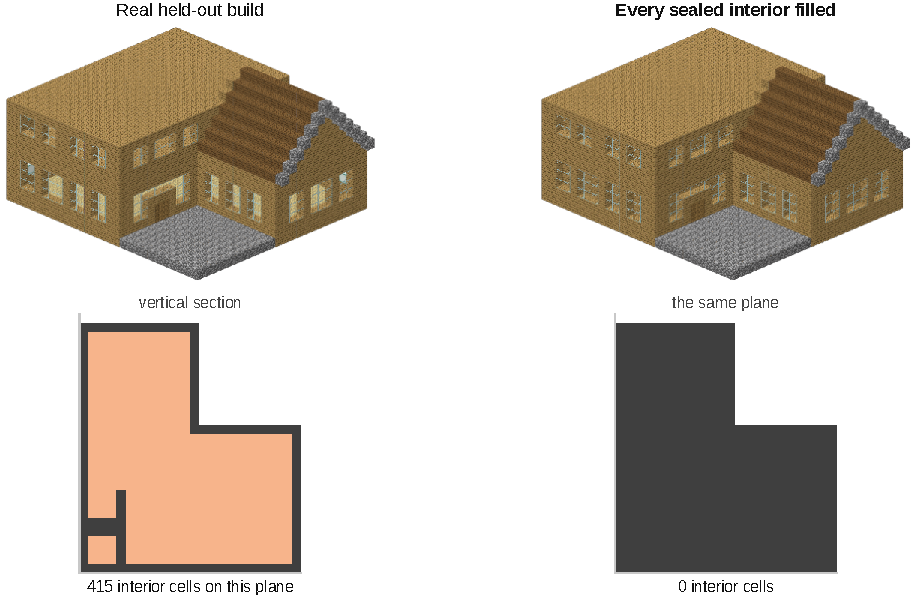
\includegraphics[width=\linewidth]{figures/fig1_teaser}
\caption{\textbf{A building is not its silhouette.} \emph{Left:} a real build, sectioned vertically through its five rooms, with sealed interior air in peach. \emph{Right:} the same build under \solidify{}, every sealed void filled by its own dominant material and cut on the same plane, almost indistinguishable in all four views the metric renders. Raw \mvkid{} moves from $-0.001$ to $+0.000$, one significance group, while \vkid{} moves $202$ noise floors. Renders use the metric's own texture pack; published builds
come from 3D-Craft (Appendix~\ref{app:data}).}
\label{fig:teaser}
\end{figure}

%TL;DR of paragraph: the probe is filling sealed interiors with the build's own material, and the render metric ties it with real data even though the metric is wide awake on the same corpus.
Our probe, \solidify{}, takes real buildings and fills every enclosed air cell with that build's own dominant material, so no new material betrays the corruption (Figure~\ref{fig:teaser}). It adds a median of $33\%$ more blocks, alters $94\%$ of examined builds, and leaves the exterior silhouette untouched. Scored at $n{=}128$ against $399$ held-out real builds, a solidified corpus and its genuine, real data counterpart \emph{share a significance group} under a paired, \com{What does this mean haha? These two last lines} Holm-corrected \citep{holm1979simple} comparison over all arm pairs. The same encoder and the same statistic separate a material permutation of the same builds at $+220.83$ noise floors (Table~\ref{tab:leaderboard}).

%TL;DR of paragraph: the cutaway ablation locates the failure in the view protocol rather than the encoder, and under an opaque renderer the invisibility is exact.
\com{weakish? Hard to follow--maybe too much bloat, see what really adds something in this paragraph}
The failure is in what the views show, not in what the encoder computes.
Holding the encoder and the statistic fixed and changing only the cameras, so
that the renders expose the interior, separates the same probe at $9$-$57$
noise floors (\S\ref{sec:ablation}). Under an opaque renderer the invisibility
is exact as filling sealed voids cannot change any
exterior view, so no encoder, statistic, sample size or view budget separates a
corpus from its solidified copy (\S\ref{sec:hollow},
Appendix~\ref{app:hull}).

%TL;DR of paragraph: the prescription is to validate a metric against corruptions of known severity before ranking with it, and to measure geometry directly alongside the renders.
\com{what does this line mean} A metric should therefore earn the right to rank. We score candidate metrics
against corruptions of known severity and require monotonicity, invariance and
sample-size stability before any of them orders a scoreboard, with separate
disqualification gates for memorization and mode collapse. Measuring geometry
directly, alongside the renders rather than instead of them, closes the blind
spot. We make three main contributions.

\begin{enumerate}[leftmargin=*,itemsep=1pt,topsep=2pt]

\item \textbf{Interior blindness, and it belongs to the representation}
(\S\ref{sec:blindness}--\ref{sec:hollow}). Render-and-embed distances cannot
distinguish a corpus of real buildings from the same corpus with every interior
filled, while the same test resolves every corruption that reaches the exterior.
Seven render-space statistics, five encoders, view budgets up to sixteen views
and a second domain all fail the same probe, and cutaway renders recover it with the same encoder
and the same statistic.

\item \textbf{A geometric metric with the complementary blindness}
(\S\ref{sec:method}). \vkid{} is a kernel distance on D4-invariant voxel
descriptors. It separates the probe by $202$ noise floors, needs no GPU, and is
\emph{exactly} invariant to material permutation, so neither metric alone ranks
both corruptions correctly.

\item \textbf{A validation protocol, and a suite that implements it}
(\S\ref{sec:method}). Gates on ordering, invariance and $n$-stability decide
whether a metric may rank anything at all. Fr\'echet distance, the functional form FID
uses, fails $n$-stability, as do coverage, recall and the biased maximum mean discrepancy
(MMD) estimator \citep{jayasumana2024cmmd}; precision and density
\citep{naeem2020prdc,kynkaanniemi2019precision} fail monotonicity.

\end{enumerate}

% \section{Related Work}
% \label{sec:related}

% \paragraph{Render-based evaluation of discrete 3D generation.}
% Recent systems for generating discrete 3D structures—including text-to-brick systems, voxel generators, and Minecraft world models—typically evaluate their outputs through rendered views. For example, Dream-Cubed \citep{merino2026dreamcubed} evaluates generated Minecraft worlds using render-based FID, while text-to-brick systems use rendered or structural representations to assess generated assemblies \citep{pun2025brickgpt,kulits2026bricknet,ni2026brickanything}. Our work does not introduce another generator or compare generation architectures; instead, we audit this shared evaluation assumption. In particular, we ask whether exterior renders expose all structural properties that an evaluation metric is expected to measure. This distinction is important because a generator can differ substantially in its hidden 3D structure while producing the same evaluated views.

% \paragraph{Alternatives to image-space evaluation.}
% A natural alternative to rendering is to evaluate generated geometry directly. Point-cloud methods compare shape distributions in geometric space \citep{achlioptas2018pointclouds}, avoiding some of the information loss introduced by projection to images. However, changing the representation does not by itself guarantee sensitivity to the property of interest. Luan et al.~\citep{luan2026rendermetric} similarly identify limitations of render-based evaluation and propose surface-point sampling to improve view coverage. Their representation remains restricted to the observed boundary: in our setting, a structure and its interior-filled counterpart have identical exterior surfaces, and therefore receive identical surface-point representations. Thus, this approach addresses incomplete \emph{view coverage} but not blindness to geometry that does not alter the exterior surface. Our geometric evaluation instead operates on volumetric structure, allowing it to detect the interior changes introduced by our controlled corruption.

% \paragraph{Auditing generative-model metrics.}
% Several works have argued that generative-model metrics should be tested for desirable properties rather than treated as universally valid measures of quality. Borji~\citep{borji2019prosandcons} identifies sensitivity to meaningful distortions and invariance to irrelevant transformations as desirable metric properties, while Chong and Forsyth~\citep{chong2020unbiasedfid} analyze the dependence of FID on sample size. O'Bray et al.~\citep{obray2022graphmetrics} provide a closer methodological precedent by applying controlled perturbations of increasing severity and testing whether a metric responds monotonically; however, they use these tests to select metric hyperparameters. We instead use controlled structural corruptions as a precondition for evaluation: a metric must demonstrate sensitivity to relevant structural changes and invariance to irrelevant ones before being used to compare generators. Herve et al.~\citep{herve2021pcgmetrics} provide a closer in-domain example of metric evaluation for procedural content generation, while Caytuiro et al.~\citep{caytuiro2025symmetry} audit whether generated structures exhibit a particular structural property. Our focus differs in that we audit the \emph{observation and representation pipeline itself}: specifically, whether an evaluation protocol can detect changes to 3D geometry that are invisible in its input views.

% \paragraph{Memorization and human evaluation.}
% Other work addresses complementary problems that arise when evaluating generative systems. Memorization can produce deceptively strong realism scores \citep{carlini2023extracting,bai2021gamedfid}, motivating nearest-neighbor retrieval and held-out comparisons for 3D generation \citep{pu2025memorization,meehan2020datacopying}. Human judgments provide another form of validation; GDMC \citep{salge2018gdmc}, for example, evaluates individual generated settlements against human-defined criteria. We adopt memorization checks as a disqualification gate; human judgment of exterior views faces the same observation limit as the metrics we audit, which is why our positive control changes the view (cutaways) rather than the judge.


\section{Related Work}
\label{sec:related}

\com{review the flow here} Recent systems for generating discrete 3D structures, including text-to-brick systems \citep{pun2025brickgpt, kulits2026bricknet, ni2026brickanything}, voxel generators \citep{chen2019voxelcnn, jung2025scaffold, awiszus2021worldgan, earle2024dreamcraft}, and Minecraft world models \citep{earle2024dreamcraft}, typically evaluate their outputs through rendered views.

\paragraph{Render-based evaluation of discrete 3D generation.}
Dream-Cubed \citep{merino2026dreamcubed}, for example, evaluates generated Minecraft worlds using render-based FID, and many text-to-brick systems use rendered or structural representations to assess generated assemblies \citep{pun2025brickgpt,kulits2026bricknet,ni2026brickanything}. FID \citep{heusel2017fid} and KID
\citep{binkowski2018kid} are the default two-sample statistics. Notably, Dream-Cubed also names the limitation we
measure in its own limitations section and reports raters agreeing with that FID only
$54.3\%$ of the time. At our sample
sizes the unbiased MMD estimator \citep{gretton2012mmd} is preferable, and
\S\ref{sec:method} shows that a widely copied biased variant ranks by sample
size instead. Precision and recall \citep{kynkaanniemi2019precision}, density
and coverage \citep{naeem2020prdc} and CMMD \citep{jayasumana2024cmmd} vary the
statistic and the features but stay in image space, so all inherit the blindness
we measure. 

%TL;DR of paragraph: siblings that generate discrete 3D structure all share the evaluation protocol we audit, and we propose no generator.
% Text-to-brick systems run language models over brick lines with a physics check
% \citep{pun2025brickgpt}, over connectivity programs \citep{kulits2026bricknet}
% and over tokenized attachment relations \citep{ni2026brickanything}. Voxel
% models predict the next block in placement order \citep{chen2019voxelcnn}, apply
% masked discrete diffusion \citep{jung2025scaffold}, fit a {3D} SinGAN
% \citep{awiszus2021worldgan} or optimize a quantized neural field per prompt
% \citep{earle2024dreamcraft}. Dream-Cubed \citep{merino2026dreamcubed} evaluates
% a controllable Minecraft world model with a render-based FID, names the limitation we
% measure in its own limitations section, and reports raters agreeing with that FID only
% $54.3\%$ of the time. 

%TL;DR of paragraph: the statistics we audit come from image generation, our geometric metric joins the point-cloud lineage, and the closest critique of rendering proposes a fix that is blind on the same axis.

\paragraph{Alternatives to image-space evaluation.}
A natural alternative to rendering is to evaluate generated geometry directly. Point-cloud methods compare shape distributions in geometric space \citep{achlioptas2018pointclouds}, avoiding some of the information loss introduced by projection to images. However, changing the representation does not by itself guarantee sensitivity to the property of interest. \citet{luan2026rendermetric} similarly identify limitations of render-based evaluation and propose surface-point sampling to improve view coverage. Their representation remains restricted to the observed boundary: in our setting, a structure and its interior-filled counterpart have identical exterior surfaces, and therefore receive identical surface-point representations. Thus, this approach addresses incomplete \emph{view coverage} but not blindness to geometry that does not alter the exterior surface. Our geometric evaluation instead operates on volumetric structure, allowing it to detect the interior changes introduced by our controlled corruption.

%TL;DR of paragraph: auditing metrics with graded perturbations is established, and we differ by making the audit blocking rather than a tuning step.
\paragraph{Auditing generative-model metrics.} Several works have argued that generative-model metrics should be tested for desirable properties rather than treated as universally valid measures of quality. \citet{borji2019prosandcons} identifies sensitivity to meaningful distortions and invariance to irrelevant transformations as desirable metric properties, while \citet{chong2020unbiasedfid} analyze the dependence of FID on sample size. 
\citet{obray2022graphmetrics} provide a closer methdological precendent by applying controlled perturbations of increasing severity and testing whether a metric responds monotonically. They use these, however, to select metric hyperparameters where we, instead, use controlled structural corruptions as a precondition for evaluation. We examine how a metric must demonstrate sensitivity to relevant structural changes and invariance to irrelevant ones before being used to compare generators. \citet{herve2021pcgmetrics} provide a closer in-domain example of metric evaluation for procedural content generation, while \citet{caytuiro2025symmetry} audit whether generated structures exhibit a particular structural property. Our focus differs in that we audit the \emph{observation and representation pipeline itself}: specifically, whether an evaluation protocol can detect changes to 3D geometry that are invisible in its input views


%TL;DR of paragraph: memorization is a documented way to win a realism leaderboard, and we adopt the retrieval protocol as a disqualification.
\paragraph{Memorization and human evaluation.} Other work addresses complementary problems that arise when evaluating generative systems. Memorization can produce deceptively strong realism scores \citep{carlini2023extracting,bai2021gamedfid}, motivating nearest-neighbor retrieval and held-out comparisons for 3D generation \citep{pu2025memorization,meehan2020datacopying}. Human judgments provide another form of validation; GDMC \citep{salge2018gdmc}, for example, evaluates individual generated settlements against human-defined criteria. We adopt memorization checks as a disqualification gate; human judgment of exterior views faces the same observation limit as the metrics we audit, which is why our positive control changes the view (cutaways) rather than the judge.

%  For {3D} shapes it is
% formalized with nearest-neighbor retrieval against a held-out baseline
% \citep{pu2025memorization,meehan2020datacopying}, which we adopt as a
% disqualification gate rather than a reported column. GDMC
% \citep{salge2018gdmc} scores settlements one build at a time against a rubric,
% whereas our metrics score \emph{distributions}. We therefore pool per-build
% two-alternative forced-choice (2AFC) judgments to the arm pair with a
% Bradley--Terry model \citep{bradley1952rank}, following current meta-evaluation
% practice \citep{deutsch2021statistical,otani2023verifiable}.

\section{Background and Problem Setting}
\label{sec:background}

%TL;DR of paragraph: notation for a structure and an arm, and the two assumptions that separate this setting from image generation.
A \emph{structure} here is a map $x : \{1,\dots,d\}^3 \to \mathcal{V}$ from a voxel grid to a
categorical block vocabulary $\mathcal{V}$, with one symbol reserved for air. An
\emph{arm} is a finite set of structures with a name and a provenance record: a
generative model's samples, a procedural generator's output, or real data under a known
corruption. Evaluation compares an arm's empirical distribution $Q$ against a fixed
reference $P$ of real structures. Two features of this setting differ from image
generation. Sample sizes are in the hundreds rather than the tens of thousands, and arms
may differ in size, so a statistic whose null depends on $n$ ranks by sample size.

%TL;DR of paragraph: define MMD, the unbiased estimator, and how KID and FID instantiate it on features.
Both metrics we report are kernel two-sample distances. For a feature map $\phi$ and a
kernel $k$,
\begin{equation}
\mathrm{MMD}^2(P,Q) = \mathbb{E}\,k(\phi(x),\phi(x')) + \mathbb{E}\,k(\phi(y),\phi(y'))
  - 2\,\mathbb{E}\,k(\phi(x),\phi(y)),
\label{eq:mmd}
\end{equation}
with $x,x' \sim P$ and $y,y' \sim Q$ \citep{gretton2012mmd}. The unbiased estimator of
Eq.~\ref{eq:mmd} omits the diagonal terms $k(\phi(x_i),\phi(x_i))$ from the within-set
means. The biased estimator keeps them, so its null on two disjoint real halves decays
with $n$. KID \citep{binkowski2018kid} is the unbiased estimator with a polynomial
kernel on encoder features, and FID \citep{heusel2017fid} fits a Gaussian to each feature
set instead. A \emph{render-and-embed} metric is any of these with $\phi =
(\text{encoder}) \circ (\text{render})$, so the structure reaches the statistic only as a
set of images. 

%TL;DR of paragraph: define the noise floor, the unit that makes metrics on different features commensurable.
Raw distances across features can differ by orders of magnitude, so we report all distances in \emph{noise floors}. For each feature and sample size $n$, the noise floor is defined as the standard deviation of the distance obtained from repeated real-vs-reference draws under the same experimental run. Thus, a value of $1.0$ indicates that the observed distance is one standard deviation of the metric's sampling variability. Because the sampling variability changes with $n$, the noise-floor unit is $n$-dependent (Appendix~\ref{app:nscale}). \com{check all appendix refs}

%TL;DR of paragraph: define the three validity properties a metric must have, which we later apply as blocking gates.
We treat a metric as \emph{valid} for ranking when it has three properties.
\begin{enumerate}
    \item 
\textbf{Ordering}: its value rises monotonically with the severity of a known corruption.
% its value rises monotonically with the severity of a corruption known to reduce quality. 
    \item \textbf{Invariance}: its value does not move under a transformation
that leaves quality unchanged. 
\item \textbf{$n$-stability}: its null on real-vs-real draws
does not drift with $n$. 
\end{enumerate}
Sensitivity, how \emph{much} damage a metric
resolves at a given $n$, is statistical power rather than measuring the right quantity, so
we record it alongside the three rather than as a fourth.

\section{Metric Validation}
\label{sec:method}

\subsection{Probes}
\label{sec:probes}

%TL;DR of paragraph: Fill-Interior fills sealed air with the build's own material, adding a third more mass behind an unchanged exterior.
\solidify{} fills every enclosed air cell of a real build with that build's own dominant
material, which keeps the silhouette bit-identical and adds only interior mass. Under a
translucent renderer it does change pixel values inside that silhouette
(\S\ref{sec:hollow}) and can only be observed externally when a structure contains this transparency (e.g. a window). On $200$ example real houses, it adds a median of $\mathbf{33\%}$
blocks (mean $37\%$) and alters $\mathbf{94\%}$ of these builds. The build's own material keeps
the corruption from showing as a palette anomaly. The probe reaches only \emph{sealed} air, air
unreachable from the bounding box without passing through solid, so air reachable through a
doorway survives; per build, the sealed share of a build's own interior volume has a median
of $100\%$ and a mean of $\mathbf{85.5\%}$ (Appendix~\ref{app:interior}).

%TL;DR of paragraph: Hollow-Shell is the exact converse probe, and four further controls damage appearance or diversity instead of geometry.
\hollow{} is the converse. It keeps a block only if one of its six faces borders air
$6$-connected to the outside, which makes it the exact set-complement of what \solidify{}
fills, and it removes a median $13.4\%$ of blocks from $98.4\%$ of builds. Four further
controls damage appearance or diversity rather than geometry. \matshuffle{} permutes the
block multiset across a build's own occupied cells, preserving geometry exactly, and
\monochrome{} repaints every block with one material. \traincopy{} (verbatim training
builds) and \singlemode{} (one build repeated $n$ times) damage nothing a distribution
distance objects to.

\subsection{MV- and K-KID}

%TL;DR of paragraph: both metrics are the same unbiased estimator and differ only in features; V-KID is a second tier, exactly material-blind and attackable.
Both realism metrics are the unbiased estimator of Eq.~\ref{eq:mmd} and differ only in
$\phi$ (Figure~\ref{fig:pipeline}). \textbf{\mvkid{}} is our stand-in for the render-and-embed family with four
orthographic views of each structure at $224$px, embedded with DINOv2-B
\citep{oquab2024dinov2}. \textbf{\vkid{}} applies the same estimator to a $77$-dimensional descriptor read
directly off the voxel grid, examining the distribution over the $55$ D4 orbits of
$2\times2\times2$ occupancy patterns, a $5$-bin wall-thickness histogram, an $8$-bin
normalized height profile, and $9$ global scalars, at about a minute per arm at $n{=}64$ on
CPU (Appendix~\ref{sec:metrics}).
\vkid{} reads occupancy only, so under
\matshuffle{} and \monochrome{} its value is \emph{bit-identical} to the real row. It measures what the render tier cannot, and not structural quality outright.

\subsection{Blocking Gates}
\label{sec:gates}

%TL;DR of paragraph: a metric failing a gate is withheld from ranking, and applying the gates to the seven statistics of tab:seven plus the biased MMD estimator settles three things.
Every candidate metric is scored on rungs of known damage, in units of its own noise
floor. A metric that fails ordering, invariance or $n$-stability is reported as
\emph{gated}, with the failing gate named, and may not rank anything. Applying this to
the seven statistics of Table~\ref{tab:seven} and the biased MMD estimator settles three
things (Appendix~\ref{app:tables}). First, we clearly see the render metric reads appearance rather than structure as \matshuffle{} preserves
geometry exactly and is yet among the worst-scoring rungs, beaten only by \monochrome{}.
Second, the biased MMD estimator is unusable at variable $n$: its null on two disjoint
real halves reads $0.289$ at $n{=}16$, $0.071$ at $n{=}64$ and $0.014$ at $n{=}400$,
while the unbiased estimator reads $0.000$ at every $n$. A leaderboard mixing arm sizes
therefore ranks by sample size. Third, precision and density fail monotonicity under
block noise, and Fr\'echet distance, recall and coverage all fail $n$-stability. Only the
unbiased KID and MMD-RBF clear each condition.

\subsection{Aggregation and Disqualification}
\label{sec:blockscore}

%TL;DR of paragraph: BlockScore is one instantiation of the gated philosophy, and the property that matters is that no pillar can be traded away.
The gates decide which metrics may speak. Turning several that pass into one ranked
number is a separate and more arbitrary problem. \blockscore{} is \emph{one} instantiation: the \textbf{maximum} over five pillars, each
divided by its own in-run scale, so there are no weights to tune. The property we defend is the maximum rather than the mean. The two tiers are
blind in complementary directions (\S\ref{sec:complementary}), so averaging lets an arm
buy a catastrophic pillar with a good one, and the trade the render tier invites is the
dangerous one: perfect surfaces over a solid interior.  Appendix~\ref{app:blockscore} records two properties of
the implementation: three of the five pillars are in true noise floors and two are in a
coarser unit that never determines the maximum, and the null of a maximum is not zero.

%TL;DR of paragraph: novelty and diversity disqualify rather than score, and every arm declares its split.
Novelty and diversity are \textbf{disqualification gates} rather than weighted terms.
An arm that trips one is refused a rank and shown with its reason, so a model cannot
offset memorization with realism. The risk is concrete here: a pre-split autoregressive
checkpoint from prior work duplicated roughly $31\%$ of training builds at intersection
over union (IoU) $\geq 0.95$. Every arm must also declare the split it trained on, the
requirement \S\ref{sec:casestudy} turns on. Gates need auditing as much as metrics do
(Appendix~\ref{app:defects}).

\section{Experimental Setup}
\label{sec:setting}

%TL;DR of paragraph: the corpus is Minecraft houses pooled from three public sources onto a shared vocabulary, and the split matters more than the pooling.
Our test medium is Minecraft houses as they represent discrete {3D} structures over a categorical block
vocabulary, at a scale where a real corpus exists and interiors are semantically
meaningful. We pool three public sources onto a shared vocabulary: a GrabCraft scrape,
the 3D-Craft house traces \citep{chen2019voxelcnn,gray2019craftassist} and the text2mc
dump. A quality gate and variant-aware deduplication leave \textbf{2{,}661} houses in a
$32^3$ box (Appendix~\ref{app:corpus}).

%TL;DR of paragraph: the split must be group-aware because public corpora ship sibling builds, and we measure the leakage a random split causes.
Public build corpora ship sibling structures, such as ``American Middle Class House 10 /
22 / 9'', and a random row split scatters a family across train and validation. Over $20$
seeds, a mean of \textbf{28.7\%} of validation items share a build family with training
(s.d.\ $2.7$, range $23.1$-$35.8$). Leakage at that rate inflates the held-out floor and
deflates every memorization statistic at once. Our canonical split is group-aware over
$2{,}054$ families at $0\%$ cross-split family overlap, pinned and released: train
$1{,}863$ / validation $399$ / test $399$. \com{what is this next line?} The calibration draw needs the same care, since
taking the first $n$ test builds rather than a shuffled sample inflates the measured noise
floor by $\mathbf{10.4\times}$ (Appendix~\ref{app:repro}).

%TL;DR of paragraph: the suite scores three kinds of arm against one fixed real reference.
The suite scores three kinds of arm against one fixed real reference
(Table~\ref{tab:arms}). \emph{Probes} are real data with a known corruption
(\S\ref{sec:probes}), \emph{baselines} are five seeded generators and
\emph{submissions} are generative models. Baselines are fitted on the training split
only, since one that had seen validation or test would hold an unearned advantage.

\begin{table}[!htb]
\centering
\scriptsize
\caption{The arms, used by these names throughout; recipes in Table~\ref{tab:arms-full}.}
\label{tab:arms}
\begin{tabular}{ll@{\hspace{1.2em}}ll}
\toprule
\multicolumn{2}{l}{\textbf{probes} (real data, corrupted)} & \multicolumn{2}{l}{\textbf{baselines} (procedural)} \\
\midrule
\realheld{}     & the floor: held-out real     & \randomvox{}   & random voxels at real density \\
\solidify{}     & every interior cell filled   & \hollowbox{}   & hollow box, walls and roof \\
\hollow{}       & interior blocks removed      & \gabled{}      & box, pitched roof, door, windows \\
\matshuffle{}   & blocks permuted, shape kept  & \patchstitch{} & $8^3$ patches, different builds \\
\monochrome{}   & one material, shape kept     & \copynoise{}   & a training build, $10\%$ displaced \\
\traincopy{}    & verbatim training copies     & \voxar{} & a native token-based model \\
\singlemode{}   & one build repeated $n$ times & \llmft{} & a finetuned language model \\
% \traincopy{}    & verbatim training copies     & \multicolumn{2}{l}{\textbf{submissions} \voxar{}, \voxarun{}, \llmft{}, \llmgeo{}} \\
% \singlemode{}   & one build repeated $n$ times & \multicolumn{2}{l}{(two token models, two language models)} \\
\bottomrule
\end{tabular}
\end{table}

%TL;DR of paragraph: what the four submissions are, and the decoding cap that limits the two language-model arms.
The four submissions are this project's own models. \voxar{} and \voxarun{} are
autoregressive transformers over merged-piece tokens, differing in whether builds are
canonically oriented. \llmft{} and \llmgeo{} are LoRA fine-tunes of a $1.5$B code model
(Qwen2.5-Coder), the second with a relative-{3D} attention bias. Both decode under a
$1200$-token cap, and \textbf{that cap limits them}: several completions are truncated
into structures one block thick (Figure~\ref{fig:samples}, Appendix~\ref{app:repro}).
They are weak baselines.

%TL;DR of paragraph: the headline configuration, the second domain, and the statistical procedure.
Every control is re-scored in every run rather than cached, because a distance means
nothing until a floor has been measured under \emph{this} run's corpus, split, $n$ and
reference size.  Unless stated otherwise,
arms are scored at $n{=}128$ against the $399$-build test reference, and significance comes
from a paired bootstrap with Holm correction \citep{holm1979simple} over all arm pairs. The
encoder ablation uses $n{=}256$ against a $512$-build reference, with the noise floor taken
from $48$ fresh real draws. The second domain is $47{,}389$ LEGO brick abstractions of
ShapeNetCore objects on a $20^3$ grid, $44\%$ of which contain a sealed void, scored at
$n{=}256$ against a $450$-build reference. Its license is unresolved, so we measure on the
corpus and publish no pictures of it (Appendix~\ref{app:data}).

\section{Results and Discussion}
\label{sec:results}

\subsection{The Render Metric Is Flat on the Interior Axis}
\label{sec:blindness}

%TL;DR of paragraph: the dose-response curve separates blindness from insensitivity, and raising n does not help.
A metric that is merely insensitive to interiors still moves when the interior changes.
\mvkid{} does not. On the occupancy-noise and mixture axes it is monotone over $121$--$143$
noise floors. On the interior axis its range end to end stays under half a noise floor, $0.48$ at
$n{=}64$ and $0.34$ at $n{=}128$, where \vkid{} reads $133$ and $287$ on the identical
rungs (Appendix~\ref{app:tables}). Raising $n$ multiplies the geometric signal by $2.2$
and does not lift the render signal off its sampling floor. Both metrics
rise on the mixture axis, a real arm progressively replaced by bad samples, which is how a
generator actually fails.

%TL;DR of paragraph: all seven render-space statistics miss the probe and catch everything else, so the blindness belongs to the representation.
Figure~\ref{fig:ladder} places both metrics on eight rungs of known damage in one run.
The flatness is not a property of the one statistic we report.
Table~\ref{tab:seven} puts seven render-space statistics on the same rungs. Six of them place the deletion of a fifth of a structure at $7$--$14$ noise
floors and one-minus-recall places it at $1.4$, while none of them places filling the
interior above $2.1$. The blindness belongs to the representation they read rather than to
any one of them.

\begin{figure}[!htb]
\centering
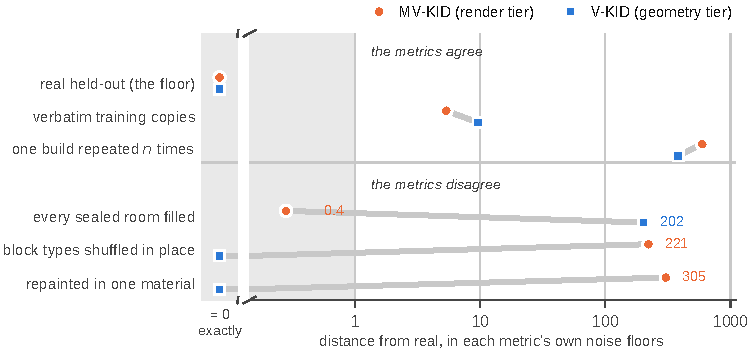
\includegraphics[width=0.88\linewidth]{figures/fig10_ladder}
\caption{\textbf{Two metrics, one run, eight rungs of known damage.} Each rung's distance
from held-out real, in that metric's own noise floors ($n{=}128$, symlog). The geometric metric's two material rungs are bit-identical to real, not merely small,
so they sit in a separate gutter. The band marks one noise floor; per-statistic numbers are in
Table~\ref{tab:seven}.}
\label{fig:ladder}
\end{figure}

\subsection{It Is the View Protocol, Not the Encoder}
\label{sec:ablation}

\begin{figure}[t]
\centering
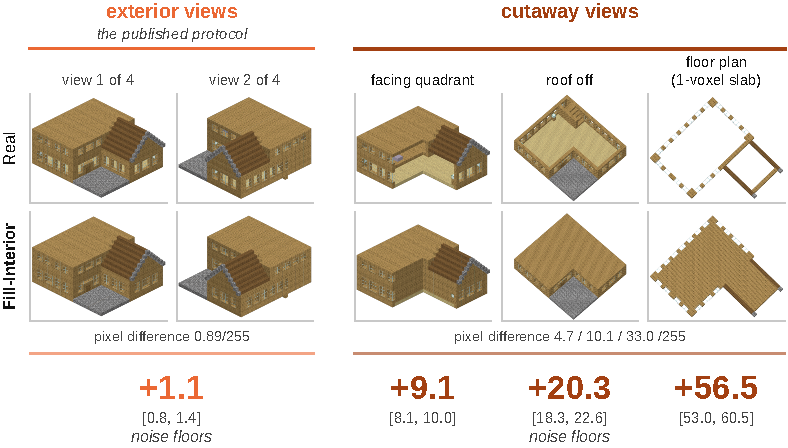
\includegraphics[width=0.90\linewidth]{figures/fig9_cutaway}
\caption{\textbf{The same encoder and statistic, only the views changed.} Each pair is a
held-out build over its \solidify{} twin. \emph{Left:} two of the four exterior views the
standard protocol renders, indistinguishable for this build at a mean pixel difference of $0.89/255$. \emph{Right:} three cutaway protocols on the same builds, each with its separation in
noise floors. DINOv2-B,
unbiased KID, $n{=}256$ against $512$ reference builds; full ablation in
Table~\ref{tab:ablation}.}
\label{fig:cutaway}
\end{figure}

%TL;DR of paragraph: varying encoder, view budget, projection and pooling changes nothing.
The finding could indict DINOv2 at four views rather than render-and-embed as a class. It
does not (Figure~\ref{fig:cutaway}, Table~\ref{tab:ablation}). Four other encoders land in the same $0.04$--$0.18$ band as our DINOv2-B: CLIP ViT-B/16 and B/32, ImageNet-supervised ResNet-50,
and the Inception network FID itself uses. Quadrupling the cameras does not help either.
\textbf{Sixteen views covering roof and underside separate the probe \emph{less} well
than four} ($+0.08$ against $+0.18$), which is what added views carrying no information about the
quantity should do. Perspective projection reads $+0.06$. Nothing measured on exterior views reaches a
quarter of one noise floor.

%TL;DR of paragraph: the cutaway rows are the positive control that makes this a statement about information rather than features.
The cutaway rows are the positive control. The same encoder and the same statistic recover
the interior at up to fifty times the separation once the view protocol stops hiding it,
which makes this a statement about \emph{information} rather than about features:
\textbf{the standard view protocol does not put interior structure into the image, so no
encoder downstream of it can score that structure.} A cutaway is not itself a good metric,
because a section view discards the facade the render tier exists to read.

\subsection{Both Directions, a Second Domain, and a Theorem}
\label{sec:hollow}

%TL;DR of paragraph: hollowing is as invisible as filling, so the blindness runs along the whole interior axis, and separations compare within a run.
The corruption this field actually produces is the converse of \solidify{}: the hollow
shells that surface-fitted mesh and implicit generators emit. It is equally invisible. In
the converse-probe run at $n{=}128$, \mvkid{} places \hollow{} at $+0.4$ noise floors and
\solidify{} at $+1.0$ against a real-vs-real floor of $+0.0$, while \vkid{} places the same
two arms at $+156.0$ and $+286.7$. The render metric is blind along the whole interior axis
rather than to one hand-built probe. Under our translucent renderer neither direction
separates at the protocol's $n{=}128$. Each run estimates its own noise floor, which is why \solidify{}
reads $286.7$ here and $201.80$ in the leaderboard run: separations compare within a run
(Appendix~\ref{app:nscale}).

%TL;DR of paragraph: the LEGO replication reproduces the qualitative structure, with the appearance controls firing on the same builds.
\label{sec:lego}The pattern is not a property of Minecraft houses. On the LEGO corpus at
$n{=}256$, with the domain pictured in Figure~\ref{fig:lego}, \mvkid{} places the solidified arm at $\mathbf{-0.01}$
noise floors, \emph{below} the real floor, while \vkid{} places it at $\mathbf{+118.6}$. On
the same builds at the same $n$ the render metric separates \matshuffle{} at
$\mathbf{+140.0}$ floors and \monochrome{} at $\mathbf{+685.8}$, so it resolves appearance
damage on this corpus and still cannot see the interior.

%TL;DR of paragraph: under an opaque renderer the invisibility is exact, which makes it a theorem rather than a measurement.
Whether interior damage reaches the image at all depends on the renderer. Under an
\emph{opaque} renderer it provably does not: filling sealed air cannot alter any exterior
view, so no encoder and no statistic can separate it at any sample size. Rendered opaquely,
all $1{,}024$ held-out (build, view) pairs we test are bit-identical, and
Appendix~\ref{app:hull} gives the proof.

%TL;DR of paragraph: our renderer leaks through translucency rather than doorways, and every changed pixel sits inside a bit-identical silhouette.
Our default renderer is not opaque, and under it \solidify{} alters $\mathbf{91\%}$ of the
$1{,}596$ test-split views, touching a median $1.2\%$ of pixels at a median maximum channel difference of $103/255$. What leaks is \emph{translucency}, not doorways:
air reachable through a doorway is never sealed, whereas a glass block in front of a filled
void does show the fill. Every changed pixel lies inside the silhouette, and the silhouette
is bit-identical (Appendix~\ref{app:hull}).

\subsection{Complementary Blindness Forces the Aggregation Rule}
\label{sec:complementary}

\begin{table}[t]
\centering
\small
\setlength{\tabcolsep}{3pt}
\caption{\textbf{The leaderboard.} Appearance and geometry are in noise floors of that pillar's own in-run real-vs-real spread, and
\blockscore{} is the \textbf{maximum} across five pillars. The three pillars that never
determine the maximum here use a coarser in-run scale and are reported in
Appendix~\ref{app:tables}. $\dagger$~marks the contaminated checkpoint of \S\ref{sec:casestudy}, unrankable and shown for comparison.}
\label{tab:leaderboard}
\begin{tabular}{rlrlrr}
\toprule
& arm & \blockscore{}~$\downarrow$ & worst pillar & appearance & geometry \\
\midrule
  & \realheld{} \emph{(anchor)}      & $0.00$   & ---        & $+0.00$   & $+0.00$ \\
\midrule
\multicolumn{6}{l}{\emph{submissions}} \\
$\dagger$ & \voxar{} \emph{(contaminated)} & $106.87$ & geometry & $+69.76$ & $+106.87$
\\
1 & \voxar{} \emph{(clean)} & $\mathbf{136.73}$ & geometry & $+85.31$ & $+136.73$ \\
2 & \llmft{} & $149.19$ & appearance & $+149.19$ & $+137.72$ \\
3 & \llmgeo{} & $191.88$ & appearance & $+191.88$ & $+145.58$ \\
4 & \patchstitch{} & $246.15$ & appearance & $+246.15$ & $+183.03$ \\
5 & \gabled{} & $300.15$ & geometry & $+287.97$ & $+300.15$ \\
6 & \hollowbox{} & $476.22$ & appearance & $+476.22$ & $+312.39$ \\
7 & \randomvox{} & $603.09$ & appearance & $+603.09$ & $+344.94$ \\
\midrule
\multicolumn{6}{l}{\emph{probes and controls: known damage, not submissions}} \\
  & \textbf{\solidify{}} & $201.80$ & geometry & $\mathbf{+0.14}$ & $\mathbf{+201.80}$ \\
  & \matshuffle{} & $231.52$ & appearance & $+231.52$ & $\mathbf{+0.00}$ \\
  & \monochrome{} & $297.95$ & appearance & $+297.95$ & $+0.00$ \\
  & \copynoise{} & $302.73$ & geometry & $+153.53$ & $+302.73$ \\
\midrule
\multicolumn{6}{l}{\emph{disqualified: refused a rank, with the reason}} \\
  & \singlemode{}                    & DQ & \multicolumn{3}{l}{mode collapse, $+45.1$ spreads on voxel diversity} \\
  & \traincopy{}                     & DQ & \multicolumn{3}{l}{memorization, $+10.7$ spreads on retrieval percentile} \\
  & \voxarun{} \emph{(clean)}        & DQ & \multicolumn{3}{l}{memorization, $+3.0$ spreads, at duplicate rate exactly $0.000$} \\
\bottomrule
\end{tabular}
\end{table}

%TL;DR of paragraph: each tier is fooled by the corruption aimed at it and rescued by the other, and the asymmetry between the two failures is large.
Table~\ref{tab:leaderboard} shows the complementarity directly. \solidify{} reads $+0.14$ on appearance against $+201.80$ on geometry, a factor of
$1{,}441$ between two pillars scoring the same arm, and \matshuffle{} is the converse,
$+231.52$ on appearance against \emph{exactly} $+0.00$ on geometry. Each tier is fooled by the corruption aimed at it and
rescued by the other, which is why \blockscore{} takes the worst pillar. The two failures
differ in severity: the best attack we have on \vkid{} is \patchstitch{}, which buys
near-perfect local occupancy statistics with globally incoherent structure and improves its geometry pillar over its appearance pillar by only $1.3\times$ ($+183.03$
against $+246.15$).

%TL;DR of paragraph: the geometric separation does not come from the added mass or from the sealed-interior scalar.
\vkid{} does not separate \solidify{} through the added mass, nor through the
sealed-interior scalar the probe drives to zero. Deleting the explicit size term moves the
separation from $201.8$ to $202.2$ floors, deleting the sealed-interior scalar moves it to
$197.1$, and deleting both leaves $197.3$. No single block of the descriptor reproduces the
result alone, the best being the scalar panel at $164.5$ (Appendix~\ref{app:descriptor}).

%TL;DR of paragraph: a mass-matched control separates on the render metric and not the geometric one, which is the dissociation stated without a probe-specific argument.
The sharper test is a control matched on the quantity in question. \growshell{} dilates the
solid outward until it has added \emph{exactly} the number of blocks \solidify{} adds to
that build, which it achieves to within one block on $128$ of $128$ builds at a median of
$196$. Same builds, same material, same mass, and the only difference is whether the new
mass goes inside or outside. The two metrics then part company completely. In that run
\mvkid{} places \growshell{} at $\mathbf{+102.3}$ noise floors and \solidify{} at
$\mathbf{+0.3}$, while \vkid{} places them at $214.5$ and $201.8$. A metric that counted
blocks could not produce that pair of rows, because the block count is the one thing the
two arms share.

%TL;DR of paragraph: the two tiers disagree about real uncorrupted builds too, and how a squared statistic is read is a separate correction.
The two tiers disagree about real, uncorrupted builds as well, with no probe involved: ranking the same $128$ held-out builds
by each metric's exact per-build contribution gives two nearly independent orderings, and
only the geometric one tracks how much interior a build has (Figure~\ref{fig:influence}).
Separately, because these statistics are squared, an arm that fails on a quarter of its
builds scores only $6.4\%$ of the way to fully bad; reporting the square root recovers the failure rate to a mean absolute error of $0.013$
against $0.128$
(Appendix~\ref{app:failrate}).

\subsection{Case Study: Contamination No Statistic Sees}
\label{sec:casestudy}

%TL;DR of paragraph: the case study asks whether the suite catches a failure we did not build, and a required provenance declaration finds it in three arms where every distribution statistic reads clean.
The results above use corruptions we built, where ground truth is known by construction.
This case study asks whether the suite catches a failure we did not build. A generator we
control is the right subject, because its training split is knowable. The suite requires
every arm to declare that split. \voxar{}, the top-ranked submission, declared one that
contained $346$ of the $399$ canonical test builds
($87\%$). \label{sec:casestudy:llm}\llmft{} and \llmgeo{} declared an earlier $90/10$
shuffle holding $53$ of the $399$ ($13\%$). No distribution statistic sees either.
\voxar{}'s duplicate rate is $0.000$ and its retrieval percentile $0.496$ against a real
held-out floor of $0.540$, far from the verbatim-copy control at $+10.7$ spreads.

%TL;DR of paragraph: retraining on the clean split erases the margin and turns the cross-track result into a tie, and the gate disqualifies the sibling checkpoint.
Retraining \voxar{} on the canonical split, with architecture and hyperparameters
unchanged, isolates the effect (Figure~\ref{fig:contamination}). We report raw \vkid{} here,
because the contaminated and clean runs do not share a noise floor. Contaminated, the arm
scores $11.62$ and separates from one language-model baseline at Holm
$5.5{\times}10^{-3}$; clean, it scores $14.898$ against their $15.006$ and $15.869$ and
separates from neither. Under a correctly calibrated test it never held a significance group
alone (Appendix~\ref{app:significance}). Contamination lowers an arm's distance from real,
so the baselines' own contamination flatters them and we report that comparison as not
separated. The gate also caught the sibling: \voxarun{}, retrained on the same clean split,
is disqualified at $+3.0$ spreads on a retrieval percentile of $0.369$ against a real floor
of $0.540$, at a duplicate rate of exactly $0.000$.

%TL;DR of paragraph: a required field beats every detector, and the two tracks fail on different pillars, which is the maximum rule acting on real submissions.
The result bears on the paper's argument twice. What detected both contaminations was a
required field rather than a detector: every memorization gate passed and the declaration
did not, so benchmarks in this domain should require that declaration and refuse to rank
arms that cannot make it. The second bearing is on aggregation. The clean \voxar{} is
geometry-limited, $+136.73$ geometry against $+79.90$ appearance, and both language-model
arms are appearance-limited, so a mean over pillars would have reported them as one model
at two quality levels (Appendix~\ref{app:tables}).

\subsection{Human Evaluation}
\label{sec:human}

%TL;DR of paragraph: the study, its three pre-registered pairs, and the exclusion rule.
Synthetic corruption shows only that the metrics order damage we built ourselves. Human
judgment is the other check. Twenty raters, naive to the hypothesis, each compared $48$ label-stripped
pairs rendered exactly as the metric renders them, yielding $912$ judgements after one
session was excluded on catch trials. Three predictions were recorded in the instrument
before any rater saw a page (Appendix~\ref{app:study}).

%TL;DR of paragraph: raters are at chance on the exterior pair and above chance on the cutaway, so the blindness is informational rather than a defect of the metric.
\textbf{The corruption is invisible to people too.} On exterior views raters preferred the
real build over its solidified copy on $43$ of $84$ trials, $0.512$ $[0.407, 0.616]$:
chance. This decides what kind of failure this is. Had people separated what the metric
could not, the metric would be failing to read something a reader reads. They cannot, so
the information is absent from the picture rather than discarded by the statistic.
\textbf{The same people separate the same builds once the view exposes the interior}, $69$
of $90$, $0.767$ $[0.669, 0.842]$, which turns ``nobody can tell'' into ``nobody can tell
\emph{from this view}''. The converse probe is also at chance, $0.606$ $[0.437, 0.753]$ on
$33$ trials.

%TL;DR of paragraph: the pre-registered pair reverses unanimously, and the geometric scalars say why.
\textbf{The pre-registered pair reversed, unanimously.} Both metrics rank \patchstitch{}
above \gabled{}; raters chose \gabled{} on \textbf{$93$ of $93$} trials $[0.960, 1.000]$.
The geometric scalars say why, and neither side is making an error. \gabled{} is a genuine
statistical outlier, a hollow and almost perfectly symmetric shell at $0.562$ open interior
ratio against a real $0.129$, so the metrics are right that it is far from the real
distribution. \patchstitch{} is assembled from patches of real builds, so its local
statistics are real by construction and only its global structure is wrong, which its
largest-connected-part ratio of $0.866$ records against a real $0.978$
(Table~\ref{tab:baselines}). A distribution distance over local features therefore rewards
\emph{statistically} house-like over \emph{recognizably} a house.

\subsection{Limitations}
\label{sec:limitations}

%TL;DR of paragraph: one renderer is the sharpest remaining gap, and the geometric tier is attackable and material-blind.
We measure two corpora and \emph{one renderer}. The renderer is the sharper gap, and the
invisibility is a
theorem about opaque rendering rather than a fact about our rasterizer
(Appendix~\ref{app:hull}), and what would close the gap is to push identical builds and the
identical probe through a path tracer sharing no code with ours. \vkid{} is a
local-statistics descriptor, and \patchstitch{}, built to exploit that, \emph{outranks} the
coherent but simple \gabled{} on both tiers, an ordering raters reverse unanimously
(\S\ref{sec:human}). That is the clearest limitation of the geometric tier, so
\patchstitch{} stays a standing control. \vkid{} is also blind to materials by
construction, which is why the suite has two tiers and neither number belongs alone.

%TL;DR of paragraph: the leaderboard runs at half the protocol's own n, and we score no published external model.
\textbf{Our own protocol asks for $n \geq 256$ and the leaderboard runs at $n{=}128$},
because the generator arms were sampled at $128$; the encoder and view ablation and the
LEGO replication are at $n{=}256$. We also score no published external model, so the
leaderboard demonstrates what the suite does rather than re-ranking a published result. The
one external comparison available without retraining is to a protocol rather than to a
model: the generator released with this corpus \citep{chen2019voxelcnn} reports a
cumulative chamfer distance, which is exactly invariant to our probe
(\S\ref{sec:related}).

\section{Conclusion}

%TL;DR of paragraph: what we found: the inherited render-and-embed protocol measures a structure's surface, so interior damage passes it untouched.
Evaluation for {3D} structure generation was inherited from image generation, and the
inheritance carries a specific defect. Rendering a structure and embedding the renders
measures its surface, and a building is not its surface. Filling every interior in a corpus
of real buildings is invisible to a multi-view kernel distance that resolves every
corruption reaching the exterior. That invisibility survives every encoder, view
budget and statistic we try, and a cutaway view removes it. Adding the same mass to the
outside of those buildings instead of the inside moves the render metric by a hundred noise
floors, so what it misses is not the quantity of the change but its location.

%TL;DR of paragraph: the general lesson, that a metric inherits the blind spots of the observation it is built on, and what follows for practice.
A metric therefore earns the right to rank models by first resolving damage of known
severity. The price is a handful of corruption arms scored beside the real reference in
every run, and what it buys is that a result resting on a blind metric fails in the lab
rather than in the literature. A metric inherits the blind spots of the observation it is
built on. A protocol that sees only what a camera sees will rank
models on the properties a camera can see, however strong the encoder behind it. Structure
that decides whether a generated object is usable, and that no camera can photograph, has
to be measured directly, and the same audit is owed to mesh and implicit {3D}
generation. \label{endofmain}

% ---------------------------------------------------------------------------
% ICLR 2027 requires an AI use statement. It does NOT count against the page
% limit, and it must be truthful: the guidelines make a misrepresentation
% produced by an LLM a Code of Ethics violation and grounds for desk rejection.
% Keep this accurate as the paper changes.
% ---------------------------------------------------------------------------
\section*{Use of Generative AI}

%TL;DR of paragraph: we disclose AI assistance by dividing the labor rather than with a blanket statement.
We used a generative AI coding assistant substantially in preparing this work,
and describe the division of labor rather than a blanket disclosure.

%TL;DR of paragraph: the assistant drafted text, figure code, parts of the suite and the literature search.
\textbf{Where it was used.} Drafting and editing the text of this paper;
implementing the figure-generation code; implementing parts of the evaluation
suite, the probes and the human-study instrument; and conducting literature
searches, including the prior-art check that identified
\citet{binkowski2018kid}'s Appendix~B.2 as the source of the mixture identity in
Appendix~\ref{app:failrate} and the limitation already stated by
\citet{merino2026dreamcubed}.

%TL;DR of paragraph: the research questions, design and interpretation are the authors', and no number came from a language model.
\textbf{Where it was not.} The research questions, the experimental design, the
decision of what to measure, and the interpretation of results are the authors'.
No experimental result, numerical value or table entry in this paper was
produced by a language model: every number is emitted by the released code from
a recorded run, and the figures read those runs directly rather than
transcribing them.

%TL;DR of paragraph: citations and arithmetic were checked, which found and fixed several errors.
\textbf{Verification.} Every citation was checked against arXiv or the official
proceedings, and every numeral in the paper is re-derived from a recorded run by a
registered check in the released code. The authors take full responsibility for the
contents of the paper, including any remaining errors.

\section*{Reproducibility Statement}

%TL;DR of paragraph: everything needed to reproduce is released, and every number is traceable to a recorded run.
The evaluation suite, probes, procedural baselines, corpus split and
human-study instrument are released. Every benchmark run writes a scorecard
recording corpus, split, sample size, reference size, seed, host, device and
commit, so each number in this paper is traceable to the run that produced it;
Appendix~\ref{app:repro} lists these. Two properties bear on replication in
particular: controls are re-scored in every run rather than cached across runs,
because the aggregate's unit is the spread of a control scored under the same
protocol; and every arm must declare the split it was trained on, with arms that
cannot reported as unranked (\S\ref{sec:casestudy}).
\TODO{Add the anonymized code URL and commit before submission, and insert the
institutional determination covering the release. The licensing question itself
is settled: Appendix~\ref{app:data} states what we redistribute and what we do
not, and the release contains no upstream content.}


\bibliography{references}
\bibliographystyle{iclr2027_conference}

\appendix
\section{Corpus Construction and Provenance}
\label{app:corpus}

\emph{Four} public sources are pooled onto a shared legacy block vocabulary
(the text2mc dump is remapped with $97\%$ block-state coverage; world cuts are
ground-stripped), passed through a quality gate, and deduplicated variant-aware.
The fourth source, \texttt{text2mc\_schem}, is the set of raw \texttt{.schem}
files in the text2mc release that its authors never converted. It entered the
pool after the $32^3$ cache was built, so that cache draws on three sources and
only the $48^3$ cache carries all four. The main text (\S\ref{sec:setting}) describes the three that build
\texttt{houses\_32}, the corpus every reported run uses.

\begin{table}[h]
\centering
\small
\caption{Corpus construction, transcribed from the cache manifests. Per-source
columns are post-gate, post-deduplication counts and sum to \textbf{final};
\textbf{final} is \emph{pooled} less \emph{drops} less \emph{dups}. Material
variants, the same shape in different materials, are \emph{kept} and not
deduplicated.}
\setlength{\tabcolsep}{4pt}
\begin{tabular}{lrrrrrrrr}
\toprule
      &        & quality & exact  &                  &           &          &         & text2mc \\
cache & pooled & drops   & dups   & \textbf{final} & GrabCraft & 3D-Craft & text2mc & \texttt{\_schem} \\
\midrule
\texttt{houses\_32} & 3{,}493 & 826 & 6 & \textbf{2{,}661} & 1{,}360 & 1{,}267 & 34 & --- \\
\texttt{houses\_48} & 4{,}502 & 1{,}381 & 33 & \textbf{3{,}088} & 1{,}410 & 1{,}381 & 180 & 117 \\
\bottomrule
\end{tabular}
\end{table}

Drop reasons at $32^3$, $826$ in total: no interior $675$, single-material blob
$52$, fragmented $37$, too flat $29$, fewer than three materials $22$, too
sparse $9$, too few blocks $2$.

\paragraph{The enclosed-air gate is calibrated per source.}
The gate requires at least $8$ interior air voxels unreachable from the bounding
box boundary. Measured on ground truth, $17\%$ of GrabCraft houses legitimately
have open interiors, against $31\%$ of 3D-Craft and $54\%$ of text2mc, so
GrabCraft is exempted from the gate and the other three are not.
\texttt{text2mc\_schem} is gated on the same grounds as the rest of the text2mc
release and is not calibrated separately. What the gate removes from the gated
sources is trees, a truck and roof fragments, read off a pre-gate visual grid.

\section{Descriptor Ablation}
\label{app:descriptor}

Two objections apply to any handcrafted descriptor. The first is that \vkid{}
separates \solidify{} only because the probe adds mass, and the descriptor
contains an explicit size term. The second is that it separates \solidify{} only
because the descriptor contains a sealed-interior scalar that the probe drives to
zero. We test both by deleting the terms and by matching the mass.

Table~\ref{tab:descriptor-ablation} reports every variant at $n{=}128$ with $48$
fresh real draws per variant, each in its own noise floor, so a column compares
variants and not raw distances. Deleting the size term \texttt{log1p\_n\_blocks}
moves the separation from $201.8$ to $202.2$. Deleting
\texttt{interior\_ratio\_sealed} moves it to $197.1$. Deleting both leaves
$197.3$. Neither term carries the result. No single block reproduces it alone
either: the strongest, the nine global scalars, reaches $164.5$ on $9$
dimensions, and the $55$ pattern bins that dominate the descriptor by dimension
reach $113.9$.

\growshell{} settles the mass question directly. It dilates the solid outward
until it has added exactly the number of blocks \solidify{} adds to that build,
which it achieves to within one block on $128$ of $128$ builds at a median of
$196$ added blocks. Same builds, same material, same mass, and the only
difference is whether the new mass lands inside or outside. The two tiers then
separate completely: \mvkid{} reads $+0.26$ noise floors on \solidify{} and
$+102.27$ on \growshell{}, while \vkid{} reads $201.8$ and $214.5$. A descriptor
that counted blocks could not produce that pair of rows.

\begin{table}[!htb]
\centering
\small
\caption{Descriptor ablation, $n{=}128$, $48$ real draws per variant. Each
separation is in that variant's own noise floor, measured under that variant.
The two suspect terms are the explicit size scalar and the sealed-interior
scalar; deleting either or both leaves the separation intact.}
\label{tab:descriptor-ablation}
\setlength{\tabcolsep}{5pt}
\begin{tabular}{lrrrr}
\toprule
descriptor variant & dims & floor & \solidify{} & \growshell{} \\
\midrule
full                              & $77$ & $0.1097$ & $\mathbf{201.8}$ & $214.5$ \\
\midrule
\multicolumn{5}{l}{\emph{deleting a suspect term}} \\
without \texttt{log1p\_n\_blocks}       & $76$ & $0.1114$ & $202.2$ & $214.9$ \\
without \texttt{interior\_ratio\_sealed}& $76$ & $0.1127$ & $197.1$ & $211.7$ \\
without both                            & $75$ & $0.1147$ & $197.3$ & $211.9$ \\
\midrule
\multicolumn{5}{l}{\emph{deleting a whole block}} \\
without pattern bins    & $22$ & $0.5113$ & $198.0$ & $120.9$ \\
without wall thickness  & $72$ & $0.1163$ & $176.4$ & $216.6$ \\
without height profile  & $69$ & $0.1312$ & $199.6$ & $213.9$ \\
without global scalars  & $68$ & $0.1302$ & $171.6$ & $206.7$ \\
\midrule
\multicolumn{5}{l}{\emph{one block alone}} \\
pattern bins only       & $55$ & $0.1802$ & $113.9$ & $201.3$ \\
wall thickness only     & $5$  & $6.0167$ & $158.7$ & $75.7$ \\
height profile only     & $8$  & $1.6293$ & $8.0$   & $28.9$ \\
global scalars only     & $9$  & $1.7594$ & $164.5$ & $118.1$ \\
\bottomrule
\end{tabular}
\end{table}


\section{Reproducibility}
\label{app:repro}

\TODO{Fill in at submission: anonymized code URL, exact commit, the pinned split
files, the feature-cache render canary hash, hardware, and per-run wall-clock.
The suite writes a scorecard carrying corpus, split, $n$, reference size, seed,
host, device and git SHA for every run, so this table is a transcription rather
than a reconstruction.}

Two properties of the protocol matter for reproducibility:

\begin{itemize}[leftmargin=*,itemsep=1pt,topsep=2pt]
\item \textbf{Controls are re-scored in every run, never cached across runs.}
  \blockscore{}'s unit is the spread of the real control \emph{scored in the
  same run}, so two scores sit on one scale only when corpus, split, tier, seed,
  reference size and control size all match. We pin these as a named protocol
  and refuse to rank runs that do not satisfy it, listing each excluded run with
  its reason. The size of the control alone moves the score: the same model on
  the same corpus, split and tier scores $87.14$ against a $128$-build control
  and $19.05$ against a $32$-build one. A board that ignored the control's size
  would read that as a $4.5\times$ improvement.
\item \textbf{The calibration draw must be shuffled.} Taking the first $n$ test
  builds as the real-vs-real draw, rather than a shuffled sample, inflates the
  measured noise floor by $\mathbf{10.4\times}$ (s.d.\ $0.0318$ against $0.0030$
  at $n{=}128$) and shifts its center from $+0.0001$ to $+0.0404$. A contiguous
  block of a corpus stored in source and family order is not an exchangeable
  sample of it, so the floor it produces is both wider and displaced, and every
  separation measured against it is understated.
\item \textbf{Every arm must declare its training split} to be ranked, and an
  arm that cannot is reported unranked with that as the stated reason. No arm in
  the run reported here declares one (\S\ref{sec:casestudy:llm}). The
  requirement post-dates that run, so it is the fix rather than a gate that
  fired.
\end{itemize}

\paragraph{The language-model arms' decoding cap.} \llmft{} and \llmgeo{} decode at
temperature $0.8$ under a $1{,}200$-token cap. That cap is a real limitation of both arms:
$11$ of $128$ generations came back empty, $139$ attempts were needed for $128$ samples,
and several completions are truncated into structures one block thick
(Figure~\ref{fig:samples}). Raising the cap requires re-running the prompts, which we did
not do for this submission.

\section{Negative Results}
\label{app:negative}

Three experiments that did not work. Each bounds a claim a reader might
otherwise expect us to make about injecting structure into sequence models.

\paragraph{Attention is not a free adjacency prior.} A pretrained code LLM's
self-attention over a serialized build recovers less adjacency information than
the coordinates already printed in the prompt. Scoring all $336$ heads by how
well they rank the truly $6$-adjacent previous pieces (AUC over the causal
candidate set), the best head reaches $0.874$ in the base model and $0.884$
after task fine-tuning, well above a recency floor. But $-\|a_i - a_j\|_1$,
three lines of arithmetic over the coordinates the serialization already prints
on every line, scores $0.980$. A trained bilinear probe does better, $0.914$ at
layer $14$ of $28$, and falls to $0.807$ by the final layer, which is the layer
generation actually reads. There is signal; there is nothing to steal.

\paragraph{A shared relative-{3D} attention bias is a null, for a reason in the
parameterization.} Adding a learned additive attention bias indexed by the
relative {3D} offset between pieces, zero-initialized and otherwise holding the
fine-tune fixed, moved best validation loss by $-0.0021$ at one seed and did not
touch the collapse mode. The learned table explains why: $364$ of $729$ offset
buckets are \emph{never updated}. Under raster emission order every earlier
piece is sign-constrained, so half the offset space is unreachable by
construction, and the arm's entire learned signal is a reparameterization of
recency. Unlocking the rest requires a non-monotonic emission order. The
reference anchor is not the constraint: the dead half of the offset space
follows from monotonic emission alone.

\section{Counting Interiors}
\label{app:interior}

A naive enclosed-air count, restricted to air cells not reachable from the
bounding-box boundary, counts a room with an open doorway as no room at all. We
additionally close
the solid under a $26$-connected morphological closing that seals openings up to
two blocks wide and report the air that becomes enclosed only then. Calibrated
on a synthetic hollow cube with a $343$-cell room: a $1{\times}1$, $1{\times}2$
or $2{\times}2$ doorway recovers all $343$ cells; a $3{\times}3$ hole or a
missing wall recovers $0$, correctly classifying an open structure as having no
room. On the same $200$ held-out houses the probe statistics of
\S\ref{sec:probes} are measured on, $\mathbf{6.0\%}$ have no \emph{sealed}
interior at all, and \emph{every one} of those twelve builds does have a room
reachable through a doorway. Pooled over builds, apertures account for
$\mathbf{25.6\%}$ of total real interior volume, which is the margin by which a
sealed-only counter understates real houses. Every claim in the earlier literature,
and in our own prior notes, that generated builds ``have no interiors'' was made
with that counter.

\paragraph{The bootstrap $p$-value floor.}
A bootstrap sign-balance $p$-value is floored at $1/n_{\text{rep}}$, and Holm
over the $55$ pairs of an $11$-arm run multiplies $0.005$ to $0.275$. Nothing
can then reach $\alpha=0.05$ however large the true difference, which put
\emph{every} arm of an earlier head-to-head, from held-out real to a monochrome
corpus, in one ``not separated'' group. The reported $p$ is now studentized and
unfloored. The failure mode is silent: it produces a table in which nothing is
significant, which reads like a careful result.

The dose axis is calibrated by construction. \textsc{Partial-Fill} fills
interior cells \emph{inward from the walls}, nearest-first, which gives an
exactly calibrated dose (interior ratio $0.1175 \to 0.0941 \to 0.0708 \to
0.0475 \to 0.0242$). Two earlier designs were rejected. Random interior speckle
is detected as \emph{noise} rather than as lost interior. Filling whole rooms
largest-first makes the axis useless, because one dominant pocket is typically
more than a quarter of the total interior, so a nominal $25\%$ dose already
removes $71\%$ of it.

\section{Defects Found in Our Own Gates}
\label{app:defects}

These are the class of error a validation ladder exists to prevent, and it did
not.

\paragraph{Two defects in our own gates.} First,
$\mathrm{sd}(\text{real})$, the unit every gate is stated in, was mismeasured
twice. It was estimated from repeated subsamples of a pool that \emph{excluded}
the probe set, so the fresh real draw being tested was not a member of its own
null. Overlapping draws also carry a finite-population factor that shrinks their
spread. Corrected, a metric that separates the solidify probe at $67$ s.d.\ passes
the gate it had failed, having been rejected for noise that was measured wrong.
Second, the $n$-stability gate tested a difference of means against the spread
of a \emph{single} draw, larger by $\sqrt{\text{reps}}$, and therefore had almost
no power. Against the standard error of the difference, the biased estimator's
$1/n$ decay is rejected at $14.8$ standard errors.

\paragraph{A third defect, in the renderer.} A feature extractor that fails
open produces numbers that look excellent and cannot be caught downstream. Ours
substituted a blank white frame for any rendering exception. Under a library
version mismatch every render raised, every image came back white, every feature
collapsed to one vector, and every arm scored KID $=-4\times 10^{-13}$, better
than real. The feature cache is validated by a render canary, so the all-white
canary would have mismatched and the cache would have been silently rebuilt from
blank frames. The renderer now raises past a $2\%$ failure rate. Repairing the
library reproduced the stored canary hash bit-for-bit, so no previously recorded
number is affected.

\section{Full Tables}
\label{app:tables}

Tables reproduced here in full, including the results the main text reports only in
prose.

\begin{table}[t]
\centering
\small
\caption{Realism at $n{=}128$ against $399$ held-out real builds, with
bootstrap $95\%$ intervals. \textbf{\solidify{} is indistinguishable from
held-out real on the render metric} and $202$ spreads away on the geometric one.
The bottom two rows are the converse blindness: \vkid{} reads occupancy only,
so a material permutation moves it by \emph{exactly} zero (values are
bit-identical to the real row, not merely close).}
\label{tab:blindness}
\begin{tabular}{lcc}
\toprule
arm & \mvkid{} $\downarrow$ & \vkid{} $\downarrow$ \\
\midrule
\realheld{} (floor)       & $-0.001$ $[-0.004, 0.003]$ & $-0.09$ $[-0.22, 0.04]$ \\
\textbf{\solidify{}}   & $\mathbf{0.000}$ $[-0.002, 0.004]$ & $\mathbf{22.03}$ $[20.65, 23.70]$ \\
\matshuffle{}& $0.674$ $[0.644, 0.712]$ & \emph{$-0.09$ (bit-identical)} \\
\monochrome{}          & $0.930$ $[0.903, 0.962]$ & \emph{$-0.09$ (bit-identical)} \\
\traincopy{}          & $0.015$ $[0.007, 0.024]$ & $0.96$ $[0.60, 1.51]$ \\
\bottomrule
\end{tabular}
\end{table}

Table~\ref{tab:blindness} is the result. The solidified corpus reads $0.000$
against a real floor of $-0.001$.

\paragraph{Significance, not interval overlap.}
Marginal confidence intervals are not a comparison, because non-overlap demands
a difference roughly $41\%$ larger than significance does. We therefore test every
arm pair with the reference draw shared and apply Holm correction
\citep{holm1979simple} across the family. Under that test
\solidify{} and \realheld{} \textbf{share a significance
group} on \mvkid{}. The same test at the same $n$ assigns
\traincopy{} its own group at a difference of $0.015$, a separation that sits on the $\alpha{=}0.05$ boundary after Holm once the test is correctly calibrated (Appendix~\ref{app:significance}), which is why the main text argues the point by magnitude instead. On \vkid{}
the same solidified arm is four groups away, $\Delta = -22.13$
$[-24.08, -20.72]$, $p \approx 0$.


\subsection{Dose--Response}

Table~\ref{tab:dose} gives every rung of the dose-response sweep, and
Figure~\ref{fig:dose} plots the three axes. Table~\ref{tab:casestudy} gives the
head-to-head letters for the case-study arms, and Figure~\ref{fig:casestudy}
plots them with bootstrap intervals.

\begin{table}[t]
\centering
\small
\caption{Dose-response, $n{=}64$ per rung. \textbf{range (sd)} is the
best-to-worst span in units of the metric's own noise floor, given as
$n{=}64$\,/\,$n{=}128$ where both were run. The render metric is perfectly
monotone on two axes and \emph{flat} on the third; on that axis its rank
correlation is unstable between the two runs ($+0.300$ vs $+0.900$), being the
correlation of a sequence that does not move, so read the span instead. A
resolution axis was dropped: changing a build's resolution changes its size, not
its quality (\S\ref{sec:setting}).}
\label{tab:dose}
\begin{tabular}{llrcr}
\toprule
axis & metric & Spearman & monotone & range (sd) \\
\midrule
\multirow{2}{*}{\textbf{solidify} (interiors filled, $0\!\to\!100\%$)}
  & \vkid{} & $+1.000$ & yes & $\mathbf{133}$\,/\,$\mathbf{287}$ \\
  & \mvkid{}   & $+0.300$\,/\,$+0.900$ & \textbf{no} & $\mathbf{0.4}$\,/\,$\mathbf{1.1}$ \\
\midrule
\multirow{2}{*}{occupancy noise ($0\!\to\!20\%$ blocks moved)}
  & \vkid{} & $+1.000$ & yes & $226$ \\
  & \mvkid{}   & $+1.000$ & yes & $143$ \\
\midrule
\multirow{2}{*}{\textbf{mixture} (fraction of arm that is real)}
  & \vkid{} & $+1.000$ & yes & $105$ \\
  & \mvkid{}   & $+1.000$ & yes & $121$ \\
\bottomrule
\end{tabular}
\end{table}


\begin{table}[t]
\centering
\small
\caption{Retraining on a clean split collapses the margin. \vkid{} at
$n{=}128$, $399$-build reference, paired and Holm-corrected over all $153$ pairs
with an exact label-permutation test. Letters mark maximal sets of arms that no
test separated at $\alpha=0.05$: a shared letter means the pair was \emph{not
separated}, never that the arms are equivalent, and an arm carries several
letters when non-separation fails to be transitive, as it does here. The
contaminated arm is not separated from either its own clean retrain or the
stronger language-model baseline, and the clean retrain ties with both baselines
it had appeared to beat.}
\label{tab:casestudy}
\begin{tabular}{llrcl}
\toprule
& arm & \vkid{} $\downarrow$ & group & status \\
\midrule
& \realheld{} (floor)      & $-0.095$ & a & --- \\
& \traincopy{}         & $0.960$  & b & DQ memorization \\
\midrule
\multirow{4}{*}{\rotatebox{90}{\footnotesize submissions}}
& \voxar{}$^{\dagger}$ \emph{(contaminated)} & $11.624$ & \textbf{d} & unranked \\
& \textbf{\voxar{}} \emph{(clean)} & $14.898$ & \textbf{def} & ranked \\
& \llmft{}            & $15.006$ & \textbf{de} & ranked \\
& \llmgeo{}               & $15.869$ & \textbf{e} & ranked \\
& \voxarun{} \emph{(clean)} & $19.570$ & fgh & \textbf{DQ memorization} \\
\midrule
& \patchstitch{}               & $19.976$ & f & ranked \\
& \randomvox{}         & $37.729$ & j & ranked \\
\bottomrule
\end{tabular}
\end{table}


\begin{table}[t]
\centering
\small
\caption{Every arm, with its full recipe. The compact version is
Table~\ref{tab:arms} in \S\ref{sec:setting}.}
\label{tab:arms-full}
\begin{tabular}{llp{7.4cm}}
\toprule
kind & name & what it is \\
\midrule
floor      & \realheld{}      & held-out real builds from the test split, disjoint from the reference they are scored against \\
\midrule
probe      & \solidify{}      & every enclosed air cell filled with the build's own dominant material \\
probe      & \matshuffle{}    & the block multiset permuted across the build's own occupied cells: geometry exactly preserved \\
probe      & \monochrome{}    & every block replaced by one material: palette destroyed, geometry exactly preserved \\
probe      & \traincopy{}     & verbatim copies of training builds \\
probe      & \singlemode{}    & one build repeated $n$ times \\
\midrule
baseline   & \randomvox{}     & random voxels at the real occupancy density \\
baseline   & \hollowbox{}     & a hollow box: floor, walls, flat roof \\
baseline   & \gabled{}        & box, pitched roof, door, windows: a competent afternoon of rules \\
baseline   & \patchstitch{}   & $8^3$ patches lifted verbatim from \emph{different} real builds \\
baseline   & \copynoise{}     & a training build with $10\%$ of its blocks displaced \\
\midrule
submission & \voxar{}         & autoregressive transformer over merged-piece tokens, trained on the canonical split \\
submission & \voxarun{}       & the same model without orientation augmentation \\
submission & \llmft{}         & a fine-tuned code language model emitting one line per piece \\
submission & \llmgeo{}        & \llmft{} with a learned relative-{3D} attention bias \\
\bottomrule
\end{tabular}
\end{table}

Every control is re-scored in every run rather than cached, because a distance
means nothing until a floor has been measured under \emph{this} run's corpus,
split, $n$ and reference size. Importing a floor across runs ranks arms against
conditions they were never measured under.

\paragraph{What is not a control.} Earlier versions of this suite
included real data requantized to a coarser grid as a ranked control. We have
removed it. Decimation changes a structure's \emph{resolution}, not its
\emph{quality}, yielding a smaller building rather than a worse one, so a
leaderboard row for it invites the comparison ``this model is worse than
$86\%$-deleted real data,'' which is not a meaningful statement about quality.
It is removed from the validation ladder for the same reason and not merely from
the leaderboard: a ladder rung asks whether a metric orders a \emph{severity}
axis correctly, and decimation is not one, so a metric that ranks it any
particular way has demonstrated nothing. No result in this paper rests on a
decimation rung.

\subsection{Metrics}
\label{sec:metrics}

We use two realism metrics throughout, both the unbiased kernel two-sample
statistic of \citet{binkowski2018kid} and differing only in the features they
are computed on.

\begin{itemize}[leftmargin=*,itemsep=1pt,topsep=2pt]
\item \textbf{\mvkid{}}, the \emph{multi-view kernel distance}. Each structure is
  rendered from four orthographic views at $224$px and embedded with DINOv2-B
  \citep{oquab2024dinov2}. This is the render-and-embed family the field uses,
  and is our stand-in for it.
\item \textbf{\vkid{}}, the \emph{voxel kernel distance}. The same estimator on a
  $77$-dimensional descriptor computed directly on the voxel grid, with no
  rendering and no GPU. The dimensions are four blocks: the distribution over
  the $\mathbf{55}$ D4-orbits of $2\times2\times2$ occupancy patterns
  ($256$ patterns fall into $55$ orbits by Burnside's lemma under the order-$8$
  group of yaw rotations and an $x$-mirror), a $\mathbf{5}$-bin wall-thickness
  histogram, an $\mathbf{8}$-bin height profile normalized by the build's own
  height, and $\mathbf{9}$ global scalars. The group is exactly D4: a vertical
  flip is deliberately \emph{not} quotiented out, since upside-down is a real
  defect in a building, and we confirm it moves $45$ of the $77$ dimensions.
  Patterns are counted over the volume padded by one air cell, so surface
  patterns are counted rather than clipped at the border. The all-empty orbit is
  identically zero after normalization, leaving $76$ informative dimensions and,
  since each of the three histograms sums to one, $73$ free parameters.
\end{itemize}

\paragraph{Whitening and clipping.} Descriptor blocks differ by orders of
magnitude in scale, so the feature map whitens against statistics frozen on the
reference, \textbf{clips at $\pm 5$ reference standard deviations}, and then
L2-normalizes each row. The clip is load-bearing rather than cosmetic and we
report it for that reason: real houses have almost no mass five voxels deep, so
the reference standard deviation of the $\text{thickness} \geq 5$ bin is
$1.6\times10^{-4}$, and \solidify{} moves that single bin by $67.5$ reference
standard deviations before clipping. Without the clip one coordinate would
dominate the kernel, and the separation we report would be a one-dimensional
thickness test wearing a $77$-dimensional coat.

Both are reported in \emph{noise floors}: the spread of repeated real-vs-reference
draws at the same $n$. A value of $1$ means one sampling-noise unit away from
real, which makes the two commensurable despite differing by three orders of
magnitude in raw units.

\subsection{Metric Validation}

Table~\ref{tab:baselines} reports the procedural baselines against real held-out data,
Figure~\ref{fig:seven} plots Table~\ref{tab:seven}, Figure~\ref{fig:gallery} shows both
probe directions on three builds,
Figure~\ref{fig:pillars} plots the two pillars against each other, and
Figure~\ref{fig:descriptor} walks through the geometric descriptor.

Every candidate metric is scored on rungs of known damage, in units of its own
noise floor (the spread of real-vs-reference draws at the same $n$). Validity
gates are \emph{blocking}: a metric that fails one is reported as \emph{gated}
with the failing gate named, and may not appear in any ranking. Sensitivity, how
\emph{much} damage a metric resolves, is recorded separately, because
that is a question about $n$, not about whether the metric measures the right
thing.

\begin{table}[t]
\centering
\small
\caption{The render tier's metric-validation ladder (DINOv2-B, $4$ orthographic
views at $224$px, $n{=}64$). Columns are the probe rungs: real held-out, retype
$10\%$ of blocks (the rung the ordering gate uses for this tier), displace
$10\%$, delete $40\%$, material shuffle and a $90^\circ$ rotation; \textbf{sd}
is the metric's own noise floor. Gates are blocking, and \emph{only \textbf{KID}
and \textbf{MMD-RBF} pass}: both PRDC recall and coverage fail $n$-stability.
MMD-RBF is on its own scale and is reported to one decimal; the last row is the
biased estimator.}
\label{tab:ladder-render}
\setlength{\tabcolsep}{3.5pt}
\begin{tabular}{lrrrrrrrl}
\toprule
       &      & retype   & displace & del.    & mat.    & rot.            & noise &      \\
metric & real & $10\%$ & $10\%$ & $40\%$ & shuffle & $90^\circ$ & floor & gate \\
\midrule
\textbf{KID} (unbiased) & \textbf{0.013} & \textbf{0.178} & \textbf{0.447} & \textbf{0.108} & \textbf{0.782} & \textbf{0.011} & \textbf{0.008} & \textbf{PASS} \\
\textbf{MMD-RBF} & \textbf{3.8} & \textbf{53.5} & \textbf{141.7} & \textbf{32.9} & \textbf{226.5} & \textbf{3.3} & \textbf{2.5} & \textbf{PASS} \\
$1-$recall & 0.113 & 0.315 & 0.919 & 0.323 & 0.750 & 0.121 & 0.027 & FAIL: $n$-stab. \\
Fr\'echet distance & 0.107 & 0.161 & 0.252 & 0.147 & 0.374 & 0.105 & 0.005 & FAIL: $n$-stab. \\
$1-$coverage & 0.258 & 0.512 & 0.839 & 0.516 & 0.952 & 0.282 & 0.052 & FAIL: $n$-stab. \\
$1-$density & 0.000 & 0.259 & 0.594 & 0.216 & 0.881 & 0.000 & 0.071 & FAIL: noise ord. \\
$1-$precision & 0.125 & 0.188 & 0.203 & 0.141 & 0.531 & 0.109 & 0.043 & FAIL: noise ord. \\
biased MMD estimator & 0.082 & 0.502 & 1.178 & 0.321 & 2.037 & 0.078 & 0.022 & FAIL: $n$-stab. \\
\bottomrule
\end{tabular}
\end{table}


\begin{table}[t]
\centering
\small
\caption{Procedural baselines, with real held-out data for reference.
\gabled{} is the bar that matters: what a competent afternoon of hand-written
rules produces. \patchstitch{} is an attack, not a baseline. Every cell is a
per-build mean over $n{=}128$ builds per baseline; the real row is all $399$
held-out test builds. \textbf{Interior is reported twice}, because the two
counters answer different questions (Appendix~\ref{app:interior}):
\emph{sealed} is air unreachable from the bounding box, \emph{open} additionally
credits rooms reachable only through a door or window. The distinction is not
cosmetic: \gabled{} has a doorway, so it scores $0.000$ sealed and $0.562$
open.}
\label{tab:baselines}
\setlength{\tabcolsep}{4pt}
\begin{tabular}{llrrrrr}
\toprule
& & & & \multicolumn{2}{c}{interior} & \\
\cmidrule(lr){5-6}
baseline & what it is & blocks & wall frac & sealed & open & LCC \\
\midrule
\randomvox{} & random voxels at real density & 1383 & 0.049 & 0.002 & 0.003 & 0.406 \\
\hollowbox{} & hollow box, floor, walls, flat roof & 1345 & 1.000 & 0.609 & 0.609 & 1.000 \\
\patchstitch{} & $8^3$ patches from \emph{different} builds & 1405 & 0.624 & 0.003 & 0.009 & 0.866 \\
\gabled{} & box, pitched roof, door, windows & 1139 & 0.969 & 0.000 & 0.562 & 1.000 \\
\copynoise{} & a training build, $10\%$ displaced & 1057 & 0.454 & 0.002 & 0.055 & 0.967 \\
\midrule
\textbf{real} & held-out test split & 924 & 0.745 & 0.114 & 0.129 & 0.978 \\
\bottomrule
\end{tabular}
\end{table}

\paragraph{Why coherence is reported as distance to real.} Two rows at the extremes of
Table~\ref{tab:leaderboard} show why the suite reports more than its two realism pillars.
An arm of \emph{verbatim copies of the training set} scores $0.015$ raw \mvkid{}, third of
sixteen arms, behind only held-out real data and \solidify{}, and only the novelty columns
catch it: nearest-neighbor IoU $1.000$, duplicate rate $1.000$ and a retrieval percentile
of $0.000$ against a real held-out floor of $0.540$. At the other end of the scale the
procedural baselines are \emph{too} hollow, with aperture-aware interior ratios of $0.61$
(\hollowbox{}) and $0.56$ (\gabled{}) against a real $0.13$. A coherence measure read as
``higher is better'' would therefore rank a hollow box above a house, which is why every
coherence measure is reported as distance to real.

\section{Human Study Protocol}
\label{app:study}

\paragraph{Protocol.} Nine arms give $36$ pairs; $288$ trials, $40$ per session,
sides randomized per trial, and arm labels stripped from the page, all enforced by an
automated check, not merely intended, because a condition visible in the DOM is
a condition the rater can read. Catch trials (real vs.\ uniform noise) are
interleaved.

\paragraph{Analysis, fixed in advance and in this order.}
\begin{enumerate}[leftmargin=*,itemsep=1pt,topsep=2pt]
\item Exclude any session scoring below $75\%$ on catch trials. A rater who
  cannot distinguish a real house from uniform noise is not doing the task, and
  the threshold is fixed here rather than tuned after seeing which exclusion
  helps a metric.
\item Fit \textbf{Bradley--Terry} arm strengths \citep{bradley1952rank} rather
  than raw win rate. Win rate depends on which opponents an arm happened to be
  drawn against, and with a random subset shown per session, coverage is always
  uneven.
\item Report (a) pairwise agreement on humanly-decided pairs and (b) Spearman
  $\rho$ against the Bradley--Terry scores. Pairs where humans are near chance
  are reported but excluded from the agreement statistic: counting them scores a
  metric on coin flips, and with enough of them any metric converges to $50\%$.
\end{enumerate}

The pipeline is validated end to end on $14$ simulated rater sessions, two of
them answering at random. It excluded exactly those two on catch
trials and recovered the injected quality ordering.

\section{Extended Related Work}
\label{app:related}

\paragraph{\citet{obray2022graphmetrics}.} Perturbs graphs at graded severity
and scores a metric on whether it responds monotonically, with Pearson
correlation against perturbation degree as the pass criterion. The procedure
selects among metric hyperparameters; it never disqualifies a metric, has no
invariance axis, and does not test stability in the sample size. Our ladder is a
blocking precondition on ranking and adds both.

\paragraph{\citet{borji2019prosandcons}.} Enumerates desiderata for generative
metrics including sensitivity to distortions, invariance to
semantically-meaningless transforms, and low sample complexity, which are our ordering,
invariance and $n$-stability gates respectively. The contribution here is
operationalizing them as a gate that runs in every evaluation rather than as a
list.

\paragraph{\citet{caytuiro2025symmetry}.} Audits {3D} generators for symmetry
violation, with the same rhetorical structure as this paper one property over.
The contrast is the point: a broken symmetry is visible in any exterior view, so
a render-and-embed metric can in principle see it. An interior cannot be seen
from outside at all, which is why the failure is structural rather than a matter
of encoder quality.

\paragraph{\citet{luan2026rendermetric}.} Criticizes rendering-based {3D}
evaluation on the grounds of incomplete structural coverage and viewpoint
sensitivity, and replaces renders with sampled surface points. This removes
rendering without removing the blindness: a surface point set describes the same
boundary. We read this as support: two independent critiques of the render
pipeline, neither of whose fixes reaches the interior.

\paragraph{\citet{herve2021pcgmetrics}.} Correlates eighteen procedural-content
metrics against GDMC jury scores. The only prior meta-evaluation of metrics in
this domain, and the precedent for validating a metric against human judgment
here rather than assuming it transfers.

\section{Full View-Protocol Ablation}

Figure~\ref{fig:ablation} plots every condition in Table~\ref{tab:ablation} on one
axis.
\label{app:ablation}

\begin{figure}[!htb]
\centering
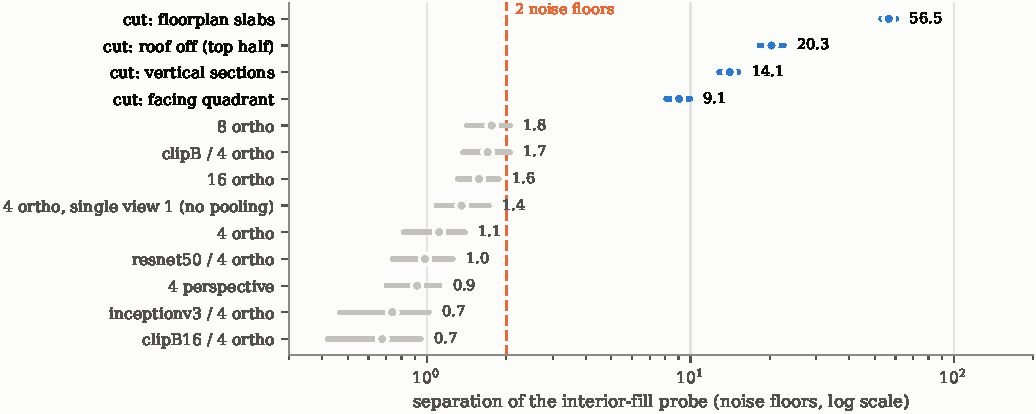
\includegraphics[width=0.9\linewidth]{figures/fig5_ablation}
\caption{\textbf{The blindness belongs to the view protocol, not the encoder.}
Separation of the interior-fill probe in each condition's own noise floors (log
scale), with paired bootstrap intervals. Gray: every encoder, view budget and
projection we test on exterior views, spanning $0.7$--$1.8$ floors. Blue: the
same encoder and the same statistic once the renders expose the interior.}
\label{fig:ablation}
\end{figure}

\begin{table}[!htb]
\centering
\small
\caption{The in-domain ladder at $n{=}128$, each statistic in its own noise floors,
measured from the floor's mean rather than from zero, so these values are not directly
comparable with Table~\ref{tab:ablation}'s. \textbf{All seven miss \solidify{} and resolve
every other corruption.}}
\label{tab:seven}
\begin{tabular}{lrrr}
\toprule
statistic & \solidify{} & $20\%$ deleted & \matshuffle{} \\
\midrule
KID & $\mathbf{2.0}$ & 12.3 & 132.3 \\
MMD-RBF & $\mathbf{2.1}$ & 13.9 & 148.8 \\
Fr\'echet distance & $\mathbf{0.5}$ & 10.8 & 72.4 \\
$1-$coverage & $\mathbf{0.2}$ & 7.7 & 19.8 \\
$1-$density & $\mathbf{0.1}$ & 7.2 & 14.0 \\
$1-$precision & $\mathbf{-0.4}$ & 9.0 & 28.0 \\
$1-$recall & $\mathbf{0.4}$ & 1.4 & 30.7 \\
\bottomrule
\end{tabular}
\end{table}

\begin{table}[!htb]
\centering
\footnotesize
\caption{Separation of \solidify{} from real in each condition's own noise floors
($n{=}256$, paired bootstrap, $95\%$ intervals). \textbf{Every exterior condition lands
between $0.7$ and $1.8$ noise floors; cutaways reach $9$--$57$ with the same encoder and
the same statistic.}}
\label{tab:ablation}
\begin{tabular}{llr@{\hspace{0.6em}}lc}
\toprule
& condition & \multicolumn{2}{c}{separation} & sees interior? \\
\midrule
\multirow{5}{*}{\rotatebox{90}{\footnotesize encoder}}
& DINOv2-B (ours) & $+1.1$ & {\footnotesize[0.8, 1.4]} & no \\
& CLIP ViT-B/16 & $+0.7$ & {\footnotesize[0.4, 0.9]} & no \\
& CLIP ViT-B/32 & $+1.7$ & {\footnotesize[1.4, 2.1]} & no \\
& ResNet-50 (ImageNet-supervised) & $+1.0$ & {\footnotesize[0.7, 1.3]} & no \\
& Inception-v3 pool3 (the FID backbone) & $+0.7$ & {\footnotesize[0.5, 1.0]} & no \\
\midrule
\multirow{3}{*}{\rotatebox{90}{\footnotesize views}}
& $8$ orthographic & $+1.8$ & {\footnotesize[1.4, 2.1]} & no \\
& $16$ orthographic & $+1.6$ & {\footnotesize[1.3, 1.9]} & no \\
& perspective & $+0.9$ & {\footnotesize[0.7, 1.1]} & no \\
\midrule
\multirow{3}{*}{\rotatebox{90}{\footnotesize \textbf{cut}}}
& \textbf{facing quadrant removed} & $\mathbf{+9.1}$ & {\footnotesize[8.1, 10.0]} & \textbf{yes} \\
& \textbf{roof removed} & $\mathbf{+20.3}$ & {\footnotesize[18.3, 22.6]} & \textbf{yes} \\
& \textbf{floorplan cross-sections} & $\mathbf{+56.5}$ & {\footnotesize[53.0, 60.5]} & \textbf{yes} \\
\midrule
& \vkid{} (no rendering at all) & $+120.8$ & {\footnotesize[115.7, 126.3]} & yes \\
\bottomrule
\end{tabular}
\end{table}

\section{What a Render Protocol Provably Cannot See}
\label{app:hull}

%TL;DR of paragraph: a deterministic renderer induces equivalence classes on which every render-and-embed metric is constant.
A deterministic render pipeline $R_V$ with a fixed view set $V$ induces an
equivalence relation on structures: $x \sim x'$ exactly when
$R_V(x) = R_V(x')$.

\begin{lemma}[Render kernel]\label{lem:kernel}
If $x \sim x'$ then $T(\mathcal{E}(R_V(x))) = T(\mathcal{E}(R_V(x')))$ for every
encoder $\mathcal{E}$, every pooling rule and every statistic $T$.
\end{lemma}
\begin{proof}
Immediate: the composition is a function of $R_V(x)$ alone.
\end{proof}

%TL;DR of paragraph: the lemma is only interesting because our own probe lands inside a class, which needs two more facts.
On its own Lemma~\ref{lem:kernel} is a tautology. It becomes a statement about
this paper because \solidify{} lands inside an equivalence class, which needs
two further facts.

\begin{lemma}[Surface invariance]\label{lem:surface}
\solidify{} leaves the exterior-air region unchanged, and leaves every exterior
face unchanged in cell, direction and material.
\end{lemma}

\begin{lemma}[Occlusion]\label{lem:occl}
Assume (a) nearest-surface shading, (b) faces bordering exterior air are opaque,
and (c) every camera lies outside the bounding box. Then
$R_V(\solidify(x)) = R_V(x)$ for \emph{every} view set $V$.
\end{lemma}
\begin{proof}[Proof sketch]
Any ray reaching a newly filled cell must first cross a face bordering exterior
air. By (b) that face is opaque and by (a) it is what the ray returns, so no
pixel can depend on the filled interior.
\end{proof}

%TL;DR of paragraph: the surface-invariance lemma also kills point-cloud and chamfer metrics, exactly.
Lemma~\ref{lem:surface} has a consequence beyond rendering. Any metric computed
on samples of the \emph{exterior surface} is a function of that face set, so it
too is constant under \solidify{}. We verify it: sampling exterior face centers
from a build and from its solidified copy gives \textbf{identical point sets on
$128$ of $128$ builds}, so chamfer distance, earth-mover distance and every
other point-cloud distance between them is exactly zero. This matters for the
proposal to replace renders with surface samples
\citep{luan2026rendermetric}, and for this corpus in particular: the model
released with it \citep{chen2019voxelcnn} reports a cumulative chamfer distance.
Sampling \emph{all} exposed faces, including those bordering sealed cavities,
does see the probe (mean chamfer $0.485$), but a surface sampler that reached
interior cavity walls would be observing the interior, which is the thing at
issue.

%TL;DR of paragraph: the conclusion, and the measurement that separates the exact regime from the leaky one.
Together with Lemma~\ref{lem:kernel} this is an impossibility result, not a
statistical one: under an opaque renderer \emph{no} encoder, statistic, sample
size or view budget separates a corpus from its solidified copy. We verify
Lemma~\ref{lem:surface} exhaustively ($0$ violations over the $399$ held-out
builds, and $0$ for \hollow{}) and Lemma~\ref{lem:occl} by rendering, using
counterfactual texture libraries to switch each hypothesis off in turn. The four
rows below are one experiment over the same $1{,}024$ (build, view) pairs, so
they are comparable to each other; the $91\%$ and $1.75\%$ quoted in
\S\ref{sec:hollow} come from a separate sweep of the whole test split
($399$ builds, $1{,}596$ views), which is why the deployed row here reads
$1.67\%$ rather than $1.75\%$. The two agree to within the difference between a
subsample and a census, and we keep each number with its own experiment rather
than mixing them:

\begin{center}\small
\begin{tabular}{lrrr}
\toprule
renderer & bit-identical & px changed (med.) & max ch.\ (med.) \\
\midrule
opaque, flat tiles (Lemma~\ref{lem:occl}) & $\mathbf{100.0\%}$ & --- & --- \\
flat tiles, translucency on & $62.5\%$ & $0.80\%$ & $94$ \\
textured, translucency off & $8.1\%$ & $0.99\%$ & $78$ \\
\textbf{deployed} (textured, translucency on) & $8.6\%$ & $1.67\%$ & $211$ \\
\bottomrule
\end{tabular}
\end{center}

%TL;DR of paragraph: our renderer violates hypothesis (b) twice, once physically and once as an artifact we disclose.
Our renderer violates hypothesis (b) in two ways, and the two have different
standing. The first is physical: Minecraft glass is translucent, so a
window in front of a filled void reveals the fill. This is a real channel, and
it is why the deployed figure is $91\%$ rather than $0\%$. The second is an
artifact of our mesh builder, which we report because it inflates that count.
\texttt{build\_mesh} assigns texture-atlas tiles in face-iteration order over
\emph{all} exposed faces, interior ones included; deleting interior faces
changes the tile count, hence the atlas layout, hence every UV rectangle, and
the sampler is nearest-neighbor. Switching translucency off still leaves $92\%$
of views altered by this alone, and within that condition ``atlas unchanged''
predicts bit-identity at $98.7\%$ agreement. A reader should therefore take
$91\%$ as a property of our renderer, not of the corruption; the corruption's
own reach is the $28\%$ that survives flattening the textures.

%TL;DR of paragraph: rescoring the probe through all four renderers shows the residual is wobble, not partial detection.
We then rescored the probe end to end through each of the four pipelines, holding
the arms, the draw and the estimator fixed and changing only the texture pack.
This turns the lemma into a prediction the benchmark either satisfies or does
not:

\begin{center}\small
\begin{tabular}{lrc}
\toprule
renderer & \mvkid{} separation & features identical \\
\midrule
opaque, flat tiles & $\mathbf{+0.000}$ & \textbf{yes} \\
flat tiles, translucency on & $-0.069$ & no \\
textured, translucency off & $+0.026$ & no \\
deployed & $+0.119$ & no \\
\bottomrule
\end{tabular}
\end{center}

The prediction holds exactly: bit-identical renders give bit-identical features
and therefore an identical kernel distance, so the separation is $0$ as an
identity rather than as a rounded measurement. The other three rows carry the
more useful lesson. The residual the benchmark reports for this probe is not a
small signal. It is \emph{wobble}. Changing only the texture pack, which
changes nothing whatever about the geometry being probed, moves it from $+0.26$
to $+0.03$ to $-0.16$: a range wider than the value itself, and one that crosses
zero, with the probe reading \emph{closer} to real than real does. This is what
it looks like when a metric is flat on an axis rather than weakly sensitive to
it, and it is why we argue the point by magnitude and ordering rather than by
the residual's sign. (The deployed row reads $+0.26$ here against the
leaderboard's $+0.38$ for the same quantity; the two runs estimate their own
floors, $0.00358$ and $0.00306$, which is the effect Appendix~\ref{app:nscale}
documents.)

%TL;DR of paragraph: where the surviving signal is lost, stated as measurement rather than theory.
Where the surviving signal dies is measurable but not, we think, provable. In
DINOv2 the patch tokens a changed pixel touches move by $0.062$ against a
between-build scale of $0.517$ ($12\%$); the CLS token moves $0.011$ against
$0.277$ ($3.9\%$); the four-view pooled embedding moves $0.0053$ against
$0.268$ ($2.0\%$). The signal enters the features and is attenuated by
aggregation. We report this as a measurement and decline the tempting story
that the encoder is invariant to the corruption by training, which the
patch-level numbers contradict.

%TL;DR of paragraph: the converse lemma, which makes the complementary-blindness claim symmetric.
The converse holds by the same style of argument and makes the paper's
complementarity claim provable on both sides rather than measured on one.

\begin{lemma}[Material blindness of \vkid{}]\label{lem:matblind}
The descriptor of \S\ref{sec:metrics} factors through the occupancy mask, so any
transformation preserving occupancy, \matshuffle{} and \monochrome{} among them,
leaves
it pointwise unchanged, and \vkid{} returns the real arm's value exactly.
\end{lemma}

Verified: descriptors are bit-identical (max difference $0.0$) and \vkid{}
returns the identical float for all three arms. The $+0.00$ printed in
Table~\ref{tab:leaderboard} is an identity, not a rounded measurement. Renders
of those same builds are never identical ($0$ of $256$ views; a median $25\%$ of
pixels move), so material permutation provably escapes the render kernel exactly
as interior fill provably falls inside it.

\section{Reading a Squared Statistic Over a Population of Prompts}
\label{app:failrate}

Everything in the main text concerns what a metric can \emph{see}. How its value is
\emph{read} is a second issue, and it affects any leaderboard reporting KID or MMD over a
population of prompts. Because these statistics are squared, an arm that fails on a quarter
of its builds scores only $6.4\%$ of the way to fully bad, where a reader assuming
proportionality would infer a quarter of the damage. Reporting the square root recovers the failure rate to a mean absolute error of $0.013$
against $0.128$ for the raw value.


A generator fails on a subset of prompts rather than uniformly. For a squared-MMD
statistic the response to such a mixture is quadratic,
\begin{equation}
\mathrm{MMD}^2\!\left(\alpha P + (1-\alpha)Q,\; P\right)
  = (1-\alpha)^2\,\mathrm{MMD}^2(Q, P),
\label{eq:mixture}
\end{equation}
a one-line consequence of the linearity of the mean embedding.
\citet{binkowski2018kid} state this identity in their Appendix B.2, and both they and
\citet{heusel2017fid} plot their metrics against a contamination fraction. We add the
reporting recommendation it implies: report $\mathrm{MMD} = \sqrt{\mathrm{MMD}^2}$, which
is \emph{linear} in the contaminated fraction and free to compute. The identity holds for
squared integral probability metrics such as KID and MMD. It does not hold for
Fr\'echet distance, which \citet{binkowski2018kid} show is not polynomial in $\alpha$,
so we derive the correction for KID only.


%TL;DR of paragraph: the measured exponent, the compression it causes, and what the square root recovers.
Measured on a mixture ladder whose bad pool is \randomvox{} at $n{=}128$, the best-fit
exponent is $\mathbf{1.99}$ against the identity's $2$. An arm failing on a quarter of
its builds scores $6.4\%$ of the way to fully bad ($0.110$ against $1.718$). Reporting
$\sqrt{\mathrm{KID}}/\sqrt{\mathrm{KID}_{\text{worst}}}$ recovers the true bad fraction
to a mean absolute error of $\mathbf{0.011}$ (\mvkid{}) and $\mathbf{0.022}$ (\vkid{}),
against $0.124$ and $0.135$ for the raw values.

%TL;DR of paragraph: the estimator is unbiased for the square, not its root, so the readout is a diagnostic rather than a ranked quantity.
One caution on the readout. The identity holds for the population quantity, while we
report an unbiased estimator of $\mathrm{MMD}^2$, which can be negative and whose square
root is therefore biased downward by Jensen's inequality, worst where the statistic is
small relative to its own standard error. We report the square root as a diagnostic for
reading a failure rate, never as the ranked quantity.

\section{What BlockScore's Maximum Is, Statistically}
\label{app:blockscore}

%TL;DR of paragraph: a max over k pillars has a positive null, so a fresh real arm scores about 1.1 rather than 0.
\blockscore{} is the maximum of five pillar scores, and a maximum of several
mean-zero quantities is not itself mean-zero. The control arm reads exactly
$0.00$ on every pillar because it \emph{is} the arm the calibration is taken
from: $(v_p - v_p)/\mathrm{sd}_p = 0$ identically, with zero variance. That is
an identity, not a measurement, and Table~\ref{tab:leaderboard} labels it as
such. A \emph{fresh} real arm, drawn from the same distribution but not used to
calibrate, scores $\mathbb{E}[\blockscore] = 1.08$ with standard deviation
$0.89$, right-skewed ($+0.89$), and a $95$th percentile of $2.8$. Read
\blockscore{} against that null rather than against zero: a value of $15$ is not
``$15$ standard deviations'' but ``far outside a null whose upper tail is under
$3$''. The inflation is about one noise floor, against a smallest ranked score
of $60.8$, so it changes no ordering and no conclusion in this paper. A
future suite comparing arms that sit within a few floors of real would need to
subtract it.

%TL;DR of paragraph: three pillars are in real noise floors and two are in a coarser unit, so the max is a veto over three.
The five pillars are not in one unit. Appearance, geometry and palette are
divided by a genuine sampling noise floor, and we verify this: their declared
units match the spread of fresh real draws to within $7\%$ ($0.93$, $1.03$ and
$1.05$ of the measured value). The coherence and geometry-scalar pillars are
divided by a per-build robust spread of the reference, an effect size measuring how
far apart two distributions are in units of how much individual builds differ
Measurement puts that unit $29\times$ and $52\times$ coarser than those
pillars' own sampling noise. A structure pillar would therefore have to move
some $1{,}800$ of its actual noise floors to veto a live pillar sitting at
$+60$, and on our card none ever does. We state this as a limitation of the
current calibration rather than a property of the aggregation rule: the maximum
is the right rule, and two of the five inputs are quoted in a unit that makes
them diagnostics rather than vetoes.

%TL;DR of paragraph: the number is only interpretable beside the name of the pillar that produced it.
One consequence for reporting. Because the winning pillar's unit is what the
number is in, \blockscore{} is uninterpretable without the pillar that produced
it, which is why every leaderboard we print carries a \emph{worst pillar}
column. It is also not convertible to a $p$-value: the null is max-shaped and
skewed, so the usual normal reading does not apply.

\section{The Noise-Floor Unit Depends on $n$}
\label{app:nscale}

Separations throughout this paper are quoted in \emph{noise floors}: the
standard deviation of repeated real-versus-reference draws at the same sample
size. That unit makes two metrics with incommensurable raw scales comparable
within a run, which is why we use it. It is not scale-free across runs,
and we state the dependence explicitly because it is easy to misread.

Measured on the identical corruption at two sample sizes:

\begin{center}
\small
\begin{tabular}{lrrrrrr}
\toprule
metric & sd $n{=}64$ & sd $n{=}128$ & ratio & sep $n{=}64$ & sep $n{=}128$ & ratio \\
\midrule
\vkid{} & 0.1732 & 0.0848 & \textbf{0.49} & 132.9 & 286.7 & \textbf{2.16} \\
\mvkid{} & 0.00449 & 0.00331 & 0.74 & 0.4 & 1.1 & 2.84 \\
\bottomrule
\end{tabular}
\end{center}

The noise floor of the geometric metric halves when $n$ doubles, the $1/n$ decay
expected of a degenerate U-statistic under the null, while the
population effect is fixed. A separation in noise floors therefore grows
\emph{linearly} in $n$, and a figure such as ``$202$'' means ``$202$ at
$n{=}128$''; the same measurement at $n{=}256$ reads roughly $400$.

Three practical consequences. Separations are only comparable across runs at
equal $n$, which is why our protocol pins it. Cross-domain figures must be
normalized before they are set side by side. And regenerating every arm at a
larger $n$ leaves the \emph{ordering} of arms intact while roughly doubling
every magnitude, and the orderings are what our conclusions rest on.

\paragraph{The unit is estimated, not only $n$-dependent, and equal $n$ is not
enough.} The floor is itself a statistic: $48$ real-versus-reference draws,
carrying a relative standard error near $1/\sqrt{2 \cdot 47} \approx 10\%$.
Two of our own runs make the consequence concrete. At the same $n{=}128$, the
same corpus, the same pinned split, the same reference and the same commit, the
leaderboard run of record reports the interior-fill separation as
$\mathbf{201.8}$ and the converse-probe run reports it as $\mathbf{286.7}$.
The only differing inputs are two random seeds, one choosing which $128$ test
builds were drawn and one seeding the $48$ floor draws. The ratio decomposes
exactly into the two:
\[
\underbrace{\frac{286.7}{201.8}}_{1.42}
\;=\;
\underbrace{\frac{0.1097}{0.0848}}_{\text{floor estimate, } 1.29}
\;\times\;
\underbrace{\frac{24.430 - 0.128}{22.034 - (-0.095)}}_{\text{raw difference, } 1.10},
\]
that is, roughly $70\%$ a different estimate of the same floor and $30\%$ a
different draw of the builds. Two estimates of one floor landing $29\%$ apart is
a $2\sigma$ event for a standard deviation taken from $48$ draws, so the unit
carries a visible error bar. A separation should therefore be read to one or two
significant figures, with its run named. We quote $202$ throughout because it is
the run of record's value, and the reader should understand it as \emph{about two
hundred}: a sweep over twelve seeds places it between $185$ and $274$.

\paragraph{The linear-in-$n$ rule holds at fixed reference size.} The
prediction above, that $n{=}256$ reads roughly $400$, assumes the reference
pool is unchanged. Our view-protocol ablation measures the same probe on the
same corpus and split at $n{=}256$ and reads $120.8$, not $400$, because it
scores against $512$ reference builds rather than $399$ and its floor
($0.188$) is consequently \emph{larger} than the $n{=}128$ floor rather than
half of it. The rule describes how a separation moves when $n$ grows within one
protocol; it does not survive a change of reference. This is the same caution as
the cross-domain one, and it is why every number in this paper is reported with
its run.

\paragraph{A note on what the ladder tables difference against.} The
per-metric ladder artifacts (Table~\ref{tab:ladder-render}) express a rung as
its distance from the null \emph{mean}, while the leaderboard expresses an arm
as its distance from a held-out \realheld{} \emph{draw}. On an exactly
invariant rung the two conventions differ by construction: the geometry metric's
material-shuffle row is $0$ exactly against the \realheld{} draw and $1.19$
against the null mean. The conventions must not be mixed within one comparison.

\mvkid{} scales less cleanly ($0.74$ rather than $0.49$) because its separation
is a ratio of two quantities that are both near zero. That is the finding rather
than a defect of the unit: the render row should be read as
``indistinguishable'', not as a number.

\section{Calibration of the Head-to-Head Test}
\label{app:significance}

%TL;DR of paragraph: the paired test we first used was anti-conservative, we replaced it with a permutation test, and we report what changed.
Our first implementation estimated the standard error of a paired difference by
subsampling $80\%$ of each arm without replacement and using the spread of those
draws directly. That is the variability of a subsample statistic around the
full-sample value, which becomes the standard error of the full-sample statistic
only after a rescale we did not apply. Measured on exact nulls, the resulting
test rejected $3.4\times$ too often at $\alpha{=}0.05$ when the arms match the
reference and $7.2\times$ too often when they do not.

%TL;DR of paragraph: no single rescale works because the statistic changes regime, so we use a permutation test.
No constant rescale repairs it. Conditional on a fixed reference, the difference
of kernel distances is a degenerate U-statistic when both arms match the
reference and a non-degenerate one when they do not, with required factors of
$1.31$ and $2.06$ respectively; across the $153$ pairs of one table the factor
ranges from $0.30$ to $11.9$. We therefore use an exact label-permutation test:
pool the two arms, re-split at the observed sizes, and recompute the difference
against the same fixed reference. Its null standard deviation tracks a
Monte-Carlo ground truth within $5\%$ in both regimes, and its type-I error is
nominal at both levels.

%TL;DR of paragraph: recomputing the run of record leaves both null results intact and costs two positive separations.
Recomputing the run of record changes only claims of separation, which is the
expected direction: a test that rejects too easily can manufacture a difference
but never a tie. Both of our null results hold and strengthen: \solidify{}
remains unseparated from held-out real ($p$ from $0.61$ to $0.77$), and the clean
retrain remains unseparated from the language-model baseline ($0.89$ to $0.93$).
Two positive separations do not survive: \traincopy{} against held-out real falls
to the $\alpha{=}0.05$ boundary, and the contaminated arm separates from one
language-model baseline but not the other. We report the blindness result by
magnitude for this reason, and the case study's conclusion, that the contaminated
arm's apparent advantage does not survive a clean split, is
unaffected, since it rests on a within-architecture comparison.

\section{Additional Figures}
\label{app:figures}

\begin{figure}[!htb]
\centering
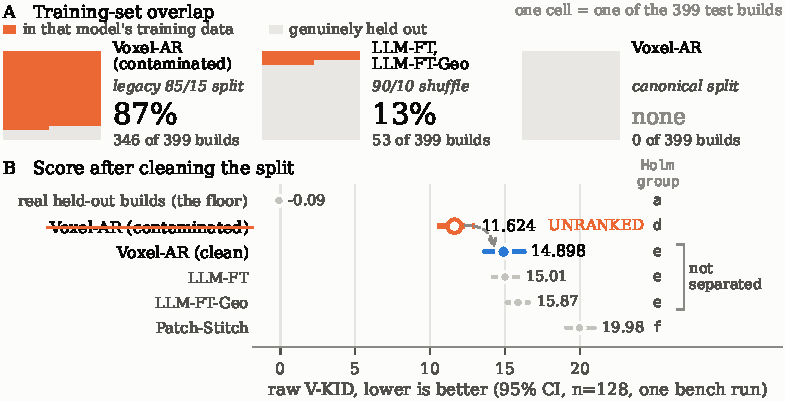
\includegraphics[width=0.90\linewidth]{figures/fig_contamination}
\caption{\textbf{Declared provenance, and what it cost.} \emph{A:} how much of the
canonical test split each arm had already trained on; the third waffle is \voxar{}
retrained on that split. \emph{B:} the retrain costs $+3.27$ raw \vkid{} and erases the
margin. No memorization gate fires on the contaminated arm, so it is unranked rather than
disqualified.}
\label{fig:contamination}
\end{figure}

\begin{figure}[!htb]
\centering
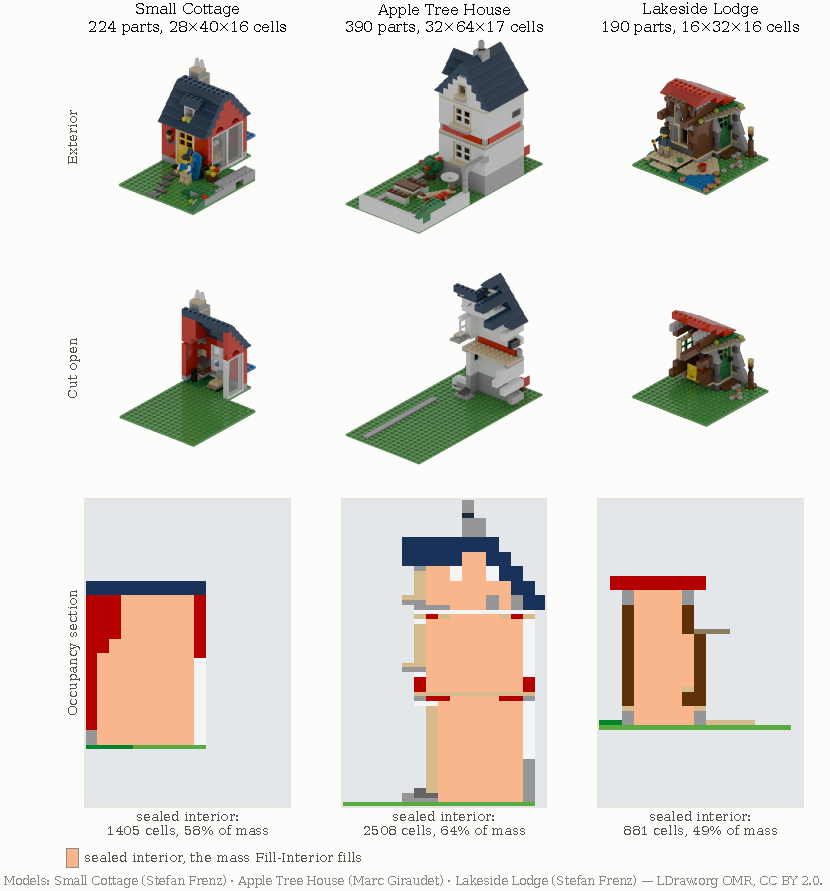
\includegraphics[width=0.72\linewidth]{figures/fig8_lego_omr}
\caption{\textbf{A second domain, with real colors.} Three LDraw.org OMR models in their
own LEGO colors: the exterior an exterior protocol sees, the same parts cut past one
plane, and the occupancy grid we derive sliced at that plane, sealed interior in peach,
every other color the parts' own, all renders at one scale. This domain shares only the
fact that builds enclose space: different parts, different lattice, different renderer, $190$--$390$ parts against
thousands of blocks. The measured replication of
\S\ref{sec:lego} runs on StableText2Brick rather than on these three models, which we
picture because their terms permit it (Appendix~\ref{app:data}). Official LEGO sets are
far less hollow than either measured corpus: among models with at least eight sealed cells,
the basis the OMR audit reports, \solidify{} adds a median $+1.2\%$ mass to an OMR model
against $+35.8\%$ to a held-out house. Models: Small Cottage (Stefan Frenz), Apple Tree House (Marc Giraudet), Lakeside
Lodge (Stefan Frenz); LDraw.org OMR, CC BY 2.0, modified only by the deletions shown.}
\label{fig:lego}
\end{figure}

\begin{figure}[!htb]
\centering
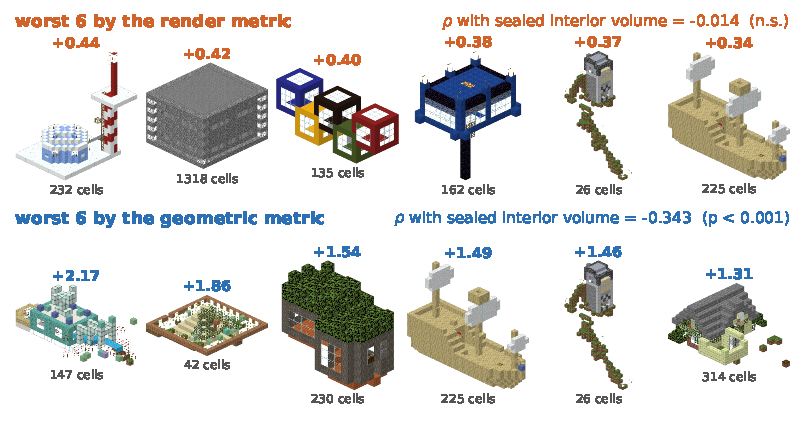
\includegraphics[width=\linewidth]{figures/fig11_influence}
\caption{\textbf{The two metrics disagree about real builds, with no probe involved.} The
unbiased estimator is a sum over builds, so each build's contribution to its arm's score is
recoverable. The six builds each metric penalizes most are shown with their contribution and
their sealed interior volume. The two orderings are nearly independent, $\rho = +0.167$, and
only the geometric ordering tracks how much interior a build has: its rank correlation with
sealed interior volume is $-0.343$ ($p < 0.001$) against $-0.014$ for the render metric.
Builds shown are 3D-Craft only, for licensing.}
\label{fig:influence}
\end{figure}

\begin{figure}[!htb]
\centering
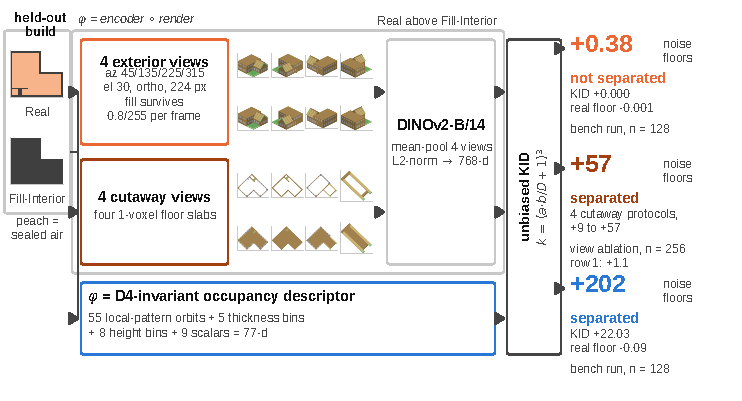
\includegraphics[width=0.95\linewidth]{figures/fig_pipeline}
\caption{\textbf{One estimator, three feature maps.} \mvkid{} and \vkid{} are the
same unbiased kernel distance of Eq.~\ref{eq:mmd} and differ only in $\phi$.
\emph{Row 1:} the render-and-embed path, where the structure reaches the statistic
as four images. \emph{Row 2:} the same renderer and the same encoder with cutaway
views, which recovers the signal. One renderer, one encoder, only the views
differ, and four other encoders and $8$ or $16$ views change nothing
(Table~\ref{tab:ablation}). \emph{Row 3:} the geometric path, which reads
occupancy directly and needs no renderer and no GPU. A noise floor is a run's own
real-vs-real spread and falls with $n$, so separations compare within a run: rows
$1$ and $3$ come from one scorecard at $n{=}128$ against $399$ reference builds,
and row $2$ from the view ablation at $n{=}256$, where row $1$ scores $+1.1$. The
sections at left are horizontal slices of one 3D-Craft build.}
\label{fig:pipeline}
\end{figure}

\begin{figure}[!htb]
\centering
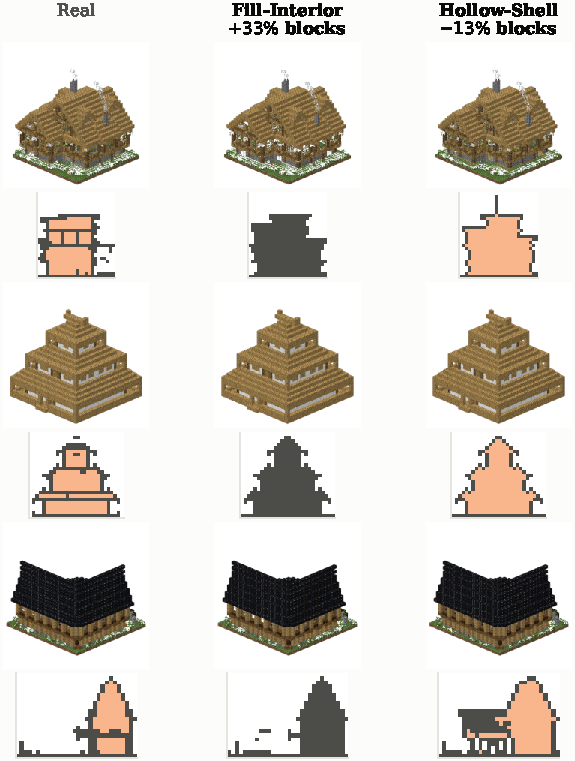
\includegraphics[width=0.60\linewidth]{figures/fig7_probe_gallery}
\caption{\textbf{Both directions of the corruption, on three held-out builds.}
\solidify{} adds a median $33\%$ blocks and \hollow{} removes a median $13\%$,
yet the views the metric is given are near-identical in every column. The
cross-sections show what changed, with sealed interior air in peach. \mvkid{} places both within one noise floor of
real ($+1.0$ and $+0.4$); \vkid{} places them $287$ and $156$ away.}
\label{fig:gallery}
\end{figure}

\begin{figure}[!htb]
\centering
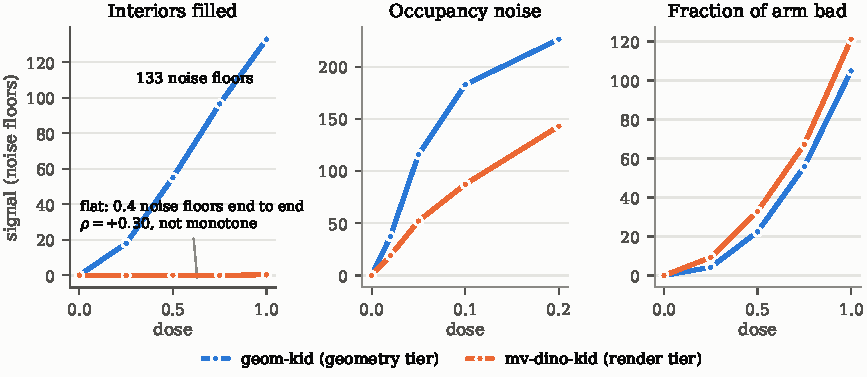
\includegraphics[width=0.95\linewidth]{figures/fig2_dose_response}
\caption{\textbf{Dose--response.} Each metric in units of its own noise floor,
which is the only scale on which the two are commensurable. Both rise
monotonically on occupancy noise and on the mixture axis; on the interior axis
the render metric does not move.}
\label{fig:dose}
\end{figure}

\begin{figure}[!htb]
\centering
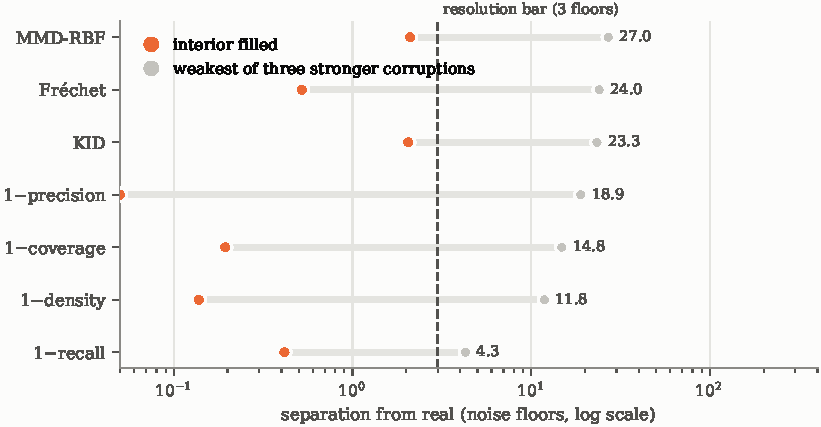
\includegraphics[width=0.86\linewidth]{figures/fig6_seven_statistics}
\caption{\textbf{Every render-space statistic shares the blindness} (LEGO,
$n{=}128$). Filled marker: the interior-fill probe. Open marker: the weakest of
three stronger corruptions. All seven resolve the stronger corruptions and none
resolves the interior fill. One minus recall also misses the milder
$20\%$-deletion rung at $1.4$ floors, a limit of that statistic rather than of
the probe.}
\label{fig:seven}
\end{figure}

\begin{figure}[!htb]
\centering
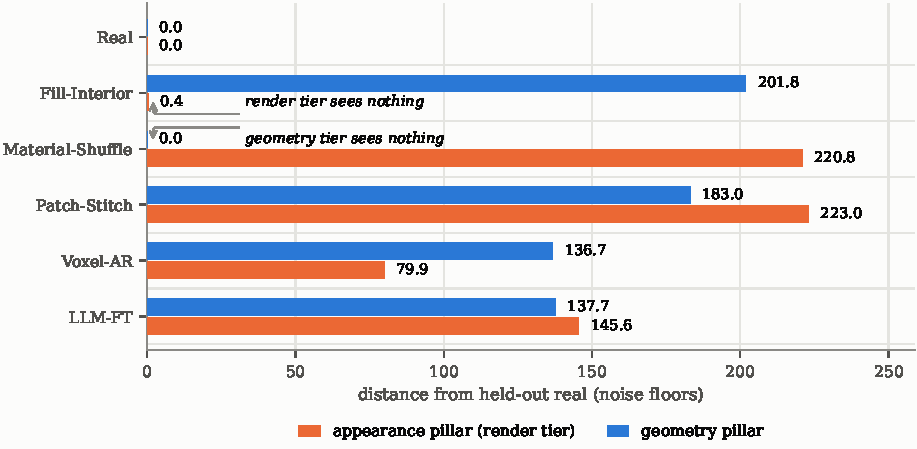
\includegraphics[width=0.88\linewidth]{figures/fig3_pillars}
\caption{\textbf{The two blindnesses are mirror images.} Distance from held-out
real on the two pillars. \solidify{} is invisible to the render tier and far from
real on geometry; \matshuffle{} is the exact converse, at precisely zero on
geometry.}
\label{fig:pillars}
\end{figure}

\begin{figure}[!htb]
\centering
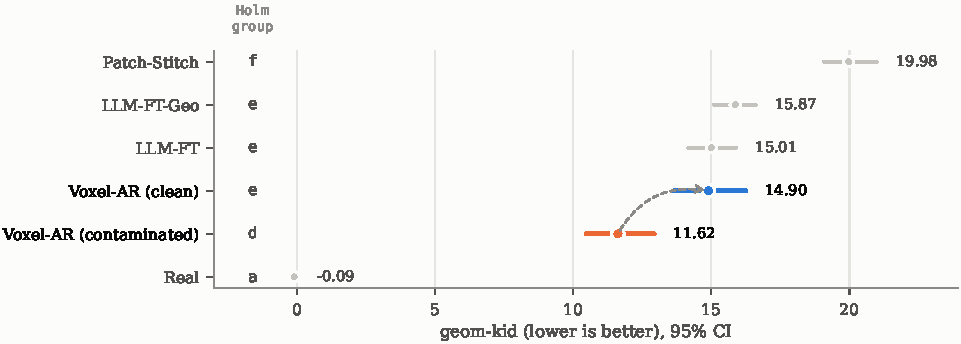
\includegraphics[width=0.9\linewidth]{figures/fig4_casestudy}
\caption{\textbf{The contamination case study.} \vkid{} with bootstrap intervals.
Cleaning the split moves \voxar{} out of group (d) and into a tie with the
baselines in group (e). The letters shown are from the original run; see
Appendix~\ref{app:significance} for the corrected compact letter display, under
which the contaminated arm does not hold a group alone.}
\label{fig:casestudy}
\end{figure}

\section{Data Provenance and Release}
\label{app:data}

%TL;DR of paragraph: what we release, what we do not, and why the corpus is reproducible without redistributing it.
Our Minecraft corpus derives from four public sources: the 3D-Craft house
dataset \citep{chen2019voxelcnn,gray2019craftassist}, released with the
CraftAssist project; a scrape of \texttt{grabcraft.com}; and the
text2mc dump, whose builds originate from \texttt{planetminecraft.com}. \textbf{We
do not redistribute the GrabCraft- or text2mc-derived structures.} GrabCraft's
terms permit sharing blueprints only by linking, and PlanetMinecraft's terms
prohibit redistributing site data. We release instead the curation code, the
per-build source URLs, content hashes, the group-aware split as index lists, and
a rebuild script, so the corpus reproduces bit-exactly without our distributing
third-party content. The four things the paper promises, namely the suite, the
probes, the baselines and the split, contain no upstream content.

%TL;DR of paragraph: published images are restricted by source, and the texture assets they use are permitted for non-commercial images but not redistributed.
Every build shown in this paper, and every stimulus shown to a human rater,
comes from \textbf{3D-Craft only}. GrabCraft's terms name pictures of blueprints
as a prohibited form of distribution; 3D-Craft's builds were commissioned as a
research corpus and carry no prohibition on depiction. Their license needs
stating precisely, because it is not the one the CraftAssist code carries. The
CraftAssist codebase is MIT, but the house data ships as a tarball with no
license file, and the release that distributes it for the 3D-Craft paper,
\texttt{facebookresearch/voxelcnn}, is CC BY-NC 4.0. We therefore treat the
corpus as non-commercial research material requiring attribution, which is what
our use and this paper's figures are, and we state that restriction on the
release rather than inheriting the code's MIT terms. Figures render these builds
with Minecraft's own texture assets, which are Mojang's copyright. Mojang's
usage guidelines permit non-commercial use of images of the game, and this
paper is non-commercial research; we also reproduce the attribution they
require, and nothing here suggests official endorsement. Two limits follow and
we observe both. The released code and data contain \textbf{no texture files},
so a reader reproducing our figures supplies them from their own installation.
And the permission covers the images, not the assets: we publish renders, never
the pack. The alternative would be flat per-block colors, which need no
permission at all because they leave only third-party-authored geometry, and
the figure scripts still produce them on request; we render with textures
because they show what the metric is actually given. Minecraft features: \copyright{} Mojang Synergies
AB, included courtesy of Mojang AB. This is not an official Minecraft product and
is not approved by or associated with Mojang or Microsoft.

%TL;DR of paragraph: attribution is by URL because creator names were never captured, and we say so.
Builds are credited by source URL in the released manifests. The original scrape
did not capture uploader names, so we cannot credit individual creators, and we
record that as a limitation rather than an omission. Our LEGO evaluation corpus
is StableText2Brick \citep{pun2025brickgpt}, loaded from HuggingFace and not
redistributed; it derives from ShapeNetCore, whose terms restrict use to
non-commercial research.
\TODO{Insert the institutional determination for the corpus release and the
human-subjects review before submission. Both are open questions for the
university's research-compliance office, not settled by the authors.}

\begin{figure}[t]
\centering
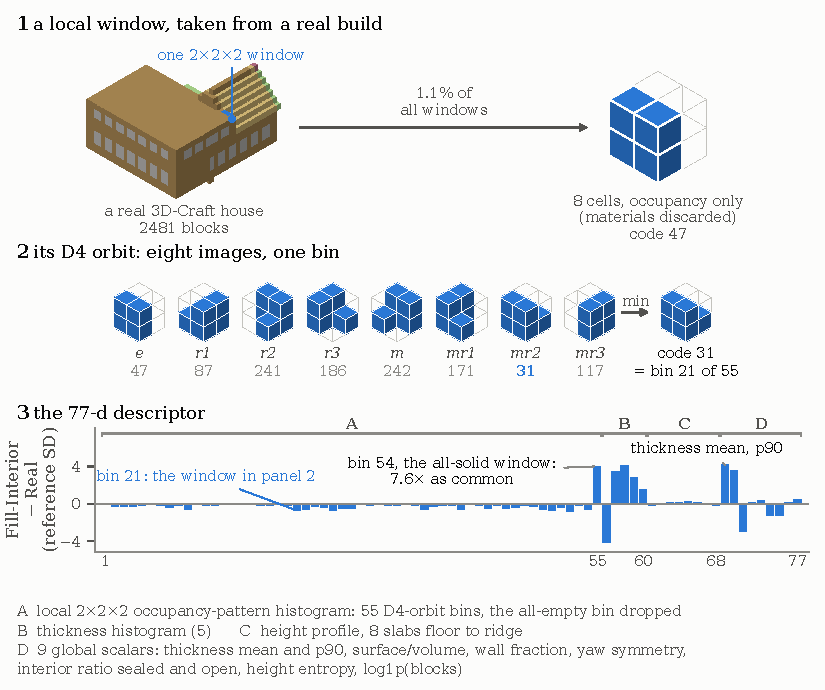
\includegraphics[width=0.92\linewidth]{figures/fig_descriptor}
\caption{\textbf{The geometric descriptor.} A $2\times2\times2$ occupancy
neighborhood, its orbit under the order-$8$ group of yaw rotations and an
$x$-mirror collapsing to one canonical bin, and the resulting feature vector with
the shift \solidify{} induces. The thickness histogram loses its one-block walls
and gains thick cores, and surface-to-volume with both interior ratios falls.
Filling every sealed interior moves this descriptor $202$ noise floors at
$n{=}128$, where the same builds move the render tier $0.4$.}
\label{fig:descriptor}
\end{figure}

\begin{figure}[p]
\centering
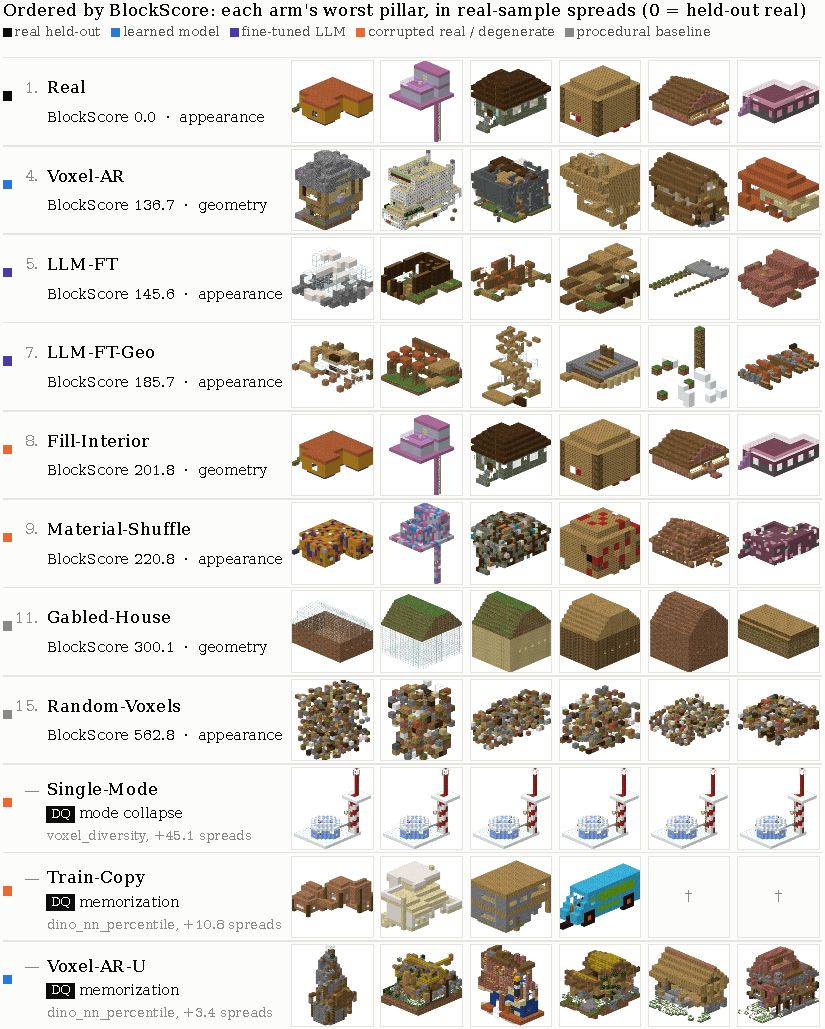
\includegraphics[width=\linewidth]{figures/fig_samples}
\caption{\textbf{Every arm, ordered by \blockscore{}.} Six builds per arm: the
first six the run recorded, in the seeded order it recorded them, topped up from
that arm's full scored sample where fewer than six remain. Builds one voxel
thick are passed over, since they draw as a hairline; a fifth of what the two
language-model arms emit is that shape, a truncation failure
\S\ref{sec:setting} describes. \realheld{}, \solidify{} and \matshuffle{} are
the same six buildings column for column, so a corruption reads down a column
and the paper's central claim can be checked by eye: the \solidify{} row scores
$+201.80$ and does not change. Each build is framed to its own bounding box, so cells are not to a common scale, and
\texttt{DQ} marks an arm a disqualification gate refused a rank
(Table~\ref{tab:leaderboard}). Cells marked $\dagger$ are withheld under
GrabCraft's terms; no build shown is a memorized copy, the nearest of $1{,}863$
training builds reaching IoU $0.51$. The contaminated checkpoint of
\S\ref{sec:casestudy} is absent: it is unrankable, and a gallery ordered by
score would imply a standing it does not have.}
\label{fig:samples}
\end{figure}


\end{document}
